\documentclass[a4paper]{book}

%General Settings
\usepackage{lmodern}
\usepackage[latin1]{inputenc}
\usepackage[T1]{fontenc}
\usepackage[english]{babel}
\usepackage{enumitem}

%Page layout
%%%Packages
\usepackage{vmargin}
\usepackage{fancyhdr}
\pagestyle{fancy}
%%%Settings
\renewcommand{\chaptermark}[1]{\markboth{#1}{}}
\renewcommand{\sectionmark}[1]{\markright{\thesection\ #1}}
\fancyhf{} \fancyhead[LE,RO]{\bfseries\thepage}
\fancyhead[RE]{\bfseries\footnotesize\nouppercase{\leftmark}}
\fancyhead[LO]{\bfseries\footnotesize\nouppercase{\rightmark}}
\setpapersize{A4}
\setmarginsrb{35mm}{10mm}{35mm}{10mm}%
             {12pt}{10mm}{5mm}{10mm}

%Crossreferences
%%%Packages
\usepackage[pdftex, bookmarks = true]{hyperref}
%%%Settings
\hypersetup{bookmarksopen = true, bookmarksopenlevel = 1, colorlinks=true,
linkcolor = black, citecolor = black, urlcolor = black, pdfstartview = FitR}

%Mathematical Fonts
\usepackage{amsfonts}
\usepackage{amsthm}
\usepackage{amssymb}
\usepackage{mathcomp}
\usepackage{mathrsfs}
\usepackage[centertags]{amsmath}
\usepackage{mathtools}
\usepackage{calligra}

\usepackage{tikz-cd}

\usepackage{microtype}

%Diagrams and Pictures
\usepackage[all,cmtip]{xy}
\usepackage{graphicx}
\usepackage{epstopdf}

%Index settings
\setcounter{tocdepth}{1}

%Bibliography settings
%%%Packages
\usepackage[style = alphabetic, backend = biber, abbreviate = true, dateabbrev = long, alldates = long]{biblatex}
%%%Settings
\renewcommand*{\newunitpunct}{\addcomma\space} %Substitutes dots (.) with commas (,)
\bibliography{Bibliography} %Path of the bibliography

%Misc Packages
\usepackage{xcolor}
\usepackage{xparse}
\usepackage{tikz}
\usepackage{comment}

%%Todo notes
%%%%Packages
\usepackage[colorinlistoftodos, textsize = small]{todonotes}
%%%%Settings
\newcounter{todocounter}
\DeclareDocumentCommand\addreference{g}{\stepcounter{todocounter}\todo[color = blue!30, fancyline]{\thetodocounter: Add reference\IfNoValueF{#1}{: #1}}}
\DeclareDocumentCommand\checkthis{g}{\stepcounter{todocounter}\todo[color = red!50, fancyline]{\thetodocounter: Check this\IfNoValueF{#1}{: #1}}}
\DeclareDocumentCommand\expandthis{g}{\stepcounter{todocounter}\todo[color = green!50, fancyline]{\thetodocounter: Expand\IfNoValueF{#1}{: #1}}}
\DeclareDocumentCommand\fixthis{g}{\stepcounter{todocounter}\todo[color = orange!50, fancyline]{\thetodocounter: Fix this\IfNoValueF{#1}{: #1}}}

%Cursive operators: sheaves Hom, Ext, Bil
%\makeatletter
%\def\@splitop#1#2\@nil{$\mathscr{#1}\!\!$\calligra#2\,\,}
%\newcommand*\DeclareCursiveOperator[2]{%
%  \newcommand#1{\mathop{\mbox{\@splitop#2\@nil}}\nolimits}}
%\makeatother
%\DeclareCursiveOperator{\EXT}{Ext}
%\DeclareCursiveOperator{\HOM}{Hom}
%\DeclareCursiveOperator{\BIL}{Bil}

%Environments
\theoremstyle{plain}
\newtheorem{thm}{Theorem}[section]
\newtheorem{theorem}[thm]{Theorem}
\newtheorem*{thm*}{Theorem}
\newtheorem{lemma}[thm]{Lemma}
\newtheorem{prop}[thm]{Proposition}
\newtheorem{proposition}[thm]{Proposition}
\newtheorem{cor}[thm]{Corollary}
\newtheorem{corollary}[thm]{Corollary}

\theoremstyle{definition}
\newtheorem{defin}[thm]{Definition}
\newtheorem{definition}[thm]{Definition}
\newtheorem{exercise}[thm]{Exercise}
\newtheorem{eg}[thm]{Example}
\newtheorem{example}[thm]{Example}

\theoremstyle{remark}
\newtheorem{rmk}[thm]{Remark}
\newtheorem{remark}[thm]{Remark}
\newtheorem*{notation}{Notation}

%Number sets, projective symbol
\newcommand{\N}{\mathbb{N}}
\newcommand{\Z}{\mathbb{Z}}
\newcommand{\Q}{\mathbb{Q}}
\newcommand{\R}{\mathbb{R}}
\newcommand{\C}{\mathbb{C}}
\newcommand{\F}{\mathbb{F}}
\newcommand{\A}{\mathbb{A}}
\newcommand{\proj}{\mathbb{P}}

%Categories
\newcommand{\Set}{\mathbf{Set}}
\newcommand{\CRing}{\mathbf{CRing}}
\newcommand{\Ab}{\mathbf{Ab}}
\newcommand{\alg}[1]{\mathbf{Alg}_#1}
\newcommand{\Top}{\mathbf{Top}}
\newcommand{\SDelta}{\mathbf \Delta}
\newcommand{\Cat}{\mathbf{Cat}}
\newcommand{\sset}{\mathbf{sSet}}
\newcommand{\ch}{\mathbf{Ch}}
\newcommand{\Ch}{\mathbf{Ch}}
\newcommand{\grpd}{\mathbf{Grpd}}
\newcommand{\Mod}{\mathbf{Mod}}
\newcommand{\cghaus}{\mathbf{CGHaus}}
\newcommand\dgCat{\ensuremath{\mathbf{dg\,Cat}}}
\DeclareDocumentCommand\dgMod{g}{\ensuremath{\IfNoValueF{#1}{#1\mhyphen}\mathbf{dg\,Mod}}}
\newcommand\sSet{\ensuremath{\simplicialCat{\Set}}}
\newcommand\simplicialCat[1]{\ensuremath{\mathbf{s\,\!#1}}}
\newcommand\simp{\ensuremath{\mathbf{s}}}
\DeclareDocumentCommand\grMod{g}{\ensuremath{\IfNoValueF{#1}{#1\mhyphen}\mathbf{gr-Mod}}}
\newcommand\Qcoh{\mathbf{Qcoh}}

%Miscellanea
\newcommand{\Hom}{\mathrm{Hom}}
\newcommand{\Ext}{\mathrm{Ext}}
\newcommand{\Tor}{\mathrm{Tor}}
\newcommand{\colim}{\mathrm{colim} \,}
\newcommand{\Max}{\mathrm{Max}}
\newcommand{\spec}{\mathrm{Spec}}
\newcommand{\Char}{\mathrm{char}}
\newcommand{\dip}{\: \mathfrak D \:}
\newcommand{\ndip}{\: \not \! \! \mathfrak D \:}
\newcommand{\trdeg}{\text{trdeg}}
\newcommand{\underscore}{\underline{\hphantom{\space{5}}}}
\newcommand{\Os}{\mathscr O}
\newcommand{\coker}{\mathrm{coker}\,}
\newcommand{\dual}{\text{\textasciicaron}}
\newcommand{\fascio}[1]{\mathscr #1}
\newcommand{\Ob}{\mathrm{Ob}}
\newcommand{\fib}{\textsc{Fib}}
\newcommand{\cofib}{\textsc{Cofib}}
\newcommand{\tot}{\mathrm{Tot}}
\newcommand{\sing}{\mathrm{Sing}}
\newcommand{\diag}{\mathrm{diag} \,}
\newcommand{\Ho}{\mathrm{Ho} \,}
\newcommand{\id}{\mathrm{id}}
\newcommand{\im}{\mathrm{Im} \,}
\newcommand{\map}{\mathrm{map}}
\newcommand{\Map}{\mathrm{Map}}
\newcommand\dash{\nobreakdash-\hspace{0pt}}
\newcommand\dd{\mathrm{d}}
\DeclareMathOperator\HH{H}
\mathchardef\mhyphen="2D
\DeclareMathOperator\Isom{Isom}
\newcommand\LLLotimes{\ensuremath{\otimes^{\mathbf{L}}}}
\newcommand\rqr{\ensuremath{\mathrm{r\,qr}}}
\newcommand\opp{\mathrm{op}}
\newcommand\RRRHHom{\ensuremath{\mathbf{R}\HHom}}
\DeclareMathOperator\HHom{\mathcal{H}om}
\DeclareMathOperator\Int{Int}
\DeclareMathOperator\ZZ{Z}
\newcommand\dg{\mathrm{dg}}
\DeclareMathOperator\KKK{\mathbf{K}}
\newcommand\unit{\mathrm{e}}
\newcommand\simeqto{\ensuremath{\mathop{\overset{\simeq}{\vphantom{\rule{0pt}{2pt}}\smash{\to}}}}}
\DeclareMathOperator\cofibrrepl{Q}
\newcommand\cof{\ensuremath{\mathrm{cof}}}
\DeclareMathOperator\nerve{N}
\DeclareMathOperator\Spec{Spec}
\newcommand\cont{\ensuremath{\mathrm{cont}}}
\newcommand\Mor{\mathrm{Mor}}
\DeclareMathOperator\RRR{\mathbf{R}}


\title{Autour de la G\'eom\'etrie Alg\'ebrique D\'eriv\'ee}
\author{Groupe de travail organis\'e par Gabriele Vezzosi \\ WORK IN PROGRESS}

\begin{document}

\frontmatter

\maketitle

\tableofcontents

%\chapter*{Introduction}
%
%The purpose of these notes is to provide a written background for the seminars taught by the working group organized by Gabriele Vezzosi in the Spring of 2013. The main goal is to give a wide introduction to Derived Algebraic Geometry, starting from the very foundations. In the present notes, we added more details with respect to the expositions, to make easier for the not (yet) specialised reader to go over them.
%
%The work is organized as follows:
%
%\begin{enumerate}
%\item Chapter 1 contains a survey of the theory of model categories: the homotopy category, function complexes, left and right (Bousfield) localizations, standard simplicial localization and hammock localization. The relative seminar has been taught the 3/15/2013 by Mauro Porta and Brice Legrignou;
%\item Chapter 2 contains a survey of all the known models for $(\infty,1)$-categories, and the details of three of those constructions (quasicategories, Segal categories and Segal spaces). The relative seminar will be taught the 3/22/2013 by Yan Zhao and Valerio Melani;
%\item Chapter 3 contains a survey of of the theory of simplicial presheaves and their application to the theory of (higher) stacks. The relative seminar has been taught the 3/29/2013 by Mauro Porta and Pietro Vertechi;
%\item
%\end{enumerate}
%
%Finally, the Appendixes contain material which is somehow more foundational: we collected some basic results from the theory of simplicial sets, enriched category theory... Essentially because the authors wanted to learn all these theories in a better way.
%
%{\bfseries This is a work in progress}

%\listoftodos
%
%\section*{Notations}
%
%\subsection*{Category Theory}
%
%$i_k \colon A_k \to A_1 \sqcup A_2$, $k = 1,2$.
%
%\subsection*{Homological Algebra}
%
%Chain complexes, $d_n \colon A_{n+1} \to A_n$.
%
%$A_\bullet$ chain complex. Then $Z_k(A_\bullet)$ and $B_k(A_\bullet)$ are cycles and boundaries.
%
%For each $n \in \N$ define $K(-,n) \colon \Mod_R \to \ch(R)$ by
%\[
%(K(A,n))_i = \begin{cases} 0 & \text{if } i \ne n \\ A & \text{if } i = n \end{cases}
%\]
%with the obvious differentials. $K(-,n)$ is clearly a functor.

\mainmatter

%\input{Model_Categories.tex}
%\chapter{Simplicial Localization}

The goal of this paper is to present the simplicial localization as defined by Dwyer ad Kan in their articles \cite{dksimplicial}, \cite{dkcomputing} and \cite{dkfunction}. The reader is supposed to know the theory of model category and homotopy category.

\begin{flushright}
Brice Le Grignou
\end{flushright}

\section{Introduction}

\subsection{Localization and higher homotopy}

Let $M$ be a model category. The axioms of model categories imply more than just homotopy relations. For example, one can describe homotopy relations between homotopy relations (see \cite[2.3]{fromHAtoHAG}). The homotopy localization loose this hidden data as it merges maps which are joined by an homotopy relation. We try here to describe this "higher homotopy structure".\\

We present first the homotopy function complexes and their relations with homotopy. Then we present the two Dwyer-Kan localizations which is the core of the paper. Finally a small theorem states that the two approach give us the same homotopy.

\subsection{Notations and terminology}

\begin{enumerate}
\item If $C$ is a category and $X,Y \in Obj(C)$, then $C(X,Y)$ denotes the set of morphisms from $X$ to $Y$ in $C$
\item If $C$ is a category, then $sC$ is the category of simplicial objects over $C$ 
\item All the categories are small (except when specified). We do not deal of set theory or universes theory issues. This is motivated by the following theorem.
\item Simplicial categories: the usual definition of a simplicial category is an enrichment over the category of simplicial set. As the categories are supposed small, one can use the following presentation:
\begin{enumerate}
\item If $A$ is a simplicial category (with small set of objects); then let $A-cat$ the category whom objects are (small) categories with $Obj(A)$ as set of objects and whom morphisms are functors which sends an object to itself.
\item Then $A$ is nothing but a simplicial object over the category $A-cat$
\end{enumerate}
\item A weak equivalence of simplicial categories $S :A \rightarrow B$ is a functor of simplicial categories such that
\begin{enumerate}
\item If $\pi_0 A$ is the category with the same objects as $A$ and such that $(\pi_0 A) (X,Y)= \pi_0 (A(X,Y))$ then $S$ induces an equivalence of (ordinary) categories $\pi_0 A \simeq \pi_0 B$ ($\pi_0 B$ is defined in the same way)
\item $A(X,Y) \rightarrow B(SX,SY)$ is a weak homotopy equivalence.
\end{enumerate}
\item In the previous definition, if $S$ is nothing but a morphism in $sA-cat$, then only the second point holds.
\item In a model category we represent the cofrations and the the fibrations by respectively: $\xymatrix{{} \ar@{^{(}->}[r] & {}}$ and $\xymatrix{{} \ar@{->>}[r] & {}}$. The weak equivalences are noted with a $\sim$.
\end{enumerate}

\begin{thm}[{\cite[Thm. 2.3]{dkfunction}}]
Let $A$ a simplicial category, and $B \in A$ a small simplicial subcategory. Then there exists a small simplicial subcategory $B'$ such that $B \subseteq B' \subseteq A$ and $B'(X,Y) \rightarrow A(X,Y)$ is a weak homotopy equivalence for all $X,Y \in B'$
\end{thm}

\section{Motivation of the simplicial localization}

\subsection{Simplicial model categories}

\begin{defin}
A simplicial model category $M$ is a model category which is also a simplicial category; this means equivalently:
\begin{enumerate}
\item $M$ is a simplicial enriched category, such as we have distinguished three classes of elements of the sets $Map(X,Y)$
\item $M$ is an element of $sM-cat$ such as $M_0$ has a model structure
\end{enumerate}
Furthermore, $M$ respects the following axioms:
\begin{enumerate}
\item For every two objects $X, Y$ of $M$, and every simplicial set $K$, there exists two objects $X\otimes K$ and $Y^K$ of $M$ such that we have isomorphisms of simplicial sets:
\begin{equation}
Map(X\otimes K, Y) \simeq Map_{sSet}(K, Map(X,Y)) \simeq Map(X, Y^K)
\end{equation}
\item If $i: A\rightarrow B$ is a cofibration in $M$ and $p:X \rightarrow Y$ is a fibration, then:
\begin{equation}
Map(B,X) \rightarrow Map(A,X) \times_{Map(A,Y)} Map(B,Y)
\end{equation}
is a fibration which is acyclic if either $i$ or $p$ is acyclic.
\end{enumerate}
\end{defin}

The simplicial model category is close to the ideal concept we want to approach from a simple model category in order to get the "higher order information" which is contained in the mapping spaces. We will see how this property happens.

\subsection{Homotopy function complexes}

Let $M$ be a model category, and $W$ a the subcategory of weak equivalence.

\begin{defin}
Let $Y$ an object of $M$. A simplicial resolution of $Y$ is a simplicial object over $M$ noted $Y_*$ together with a weak equivalence $Y \rightarrow Y_0$ such that
\begin{enumerate}
\item the object $Y_0$ is fibrant
\item all faces maps in $Y_*$ are acyclic fibrations. Hence, all the objects $Y_n$ are fibrants.
\item Let $(d_*, Y_n)$ the diagram:
\begin{enumerate}
\item for every $0 \le i \le n+1$, a copy $(d_i; Y_n)$ of $Y_n$
\item for every $0 \le i < j \le n+1$, a copy $(d_id_j,Y_{n-1})$ of $Y_{n-1}$
\item pair of maps: $(d_j, Y_n) \rightarrow (d_id_j,Y_{n-1}) \leftarrow (d_j, Y_n)$. These arrows are acyclic fibrations. 
\end{enumerate}
Then the map $Y_{n+1} \rightarrow (d_*,Y_n)$ is a fibration.
\end{enumerate}
\end{defin}

\begin{defin}
A simplicial resolution $Y_*$ of $Y$ can be viewed as a simplicial object over $M$ together with a simplicial map $i:Y \rightarrow Y_*$ (here $Y$ represents the constant simplicial object over $M$ made from the object $Y$), and having some further properties. Then one can define a map of simplicial resolutions of $Y$, $f:Y_* \rightarrow {Y'}_*$ as a simplicial map which makes the following diagram commute:
\[ \xymatrix{Y \ar[rr] \ar[dr] && {Y'_*} \\ & Y \ar[ur]} \]
\end{defin}


\begin{defin}
The notion of cosimplicial resolution and map between cosimplicial resolutions are defined dually from the notion of simplicial resolution and map of simplicial resolutions.
\end{defin}

With these notions, one can try to state the definition:

\begin{defin}
$M(X^*,Y_*)$ has an obvious structure of bisimplicial set for $X^*$ a cosimplicial resolution of $X$ and $Y_*$ a simplicial resolution of $Y$. The homotopy complex of $(X,Y)$ is then defined as $diag M(X^*,Y_*)$ .
\end{defin}

However, one needs some machinery to make this definitions coherent. Indeed one has to check that the homotopy can be defined for two objects $(X,Y)$ and that it does not depens on the resolutions chosed. The first requirement is answered by: 

\begin{prop}
Every object of a model category $M$ has simplicial and a cosimplicial resolutions.
\end{prop}

\begin{proof}
Let's show the result by induction for a simplicial resolution. One adds a requirement of this simplicial resolution (usefull for the construction): the degeneracies are acyclic cofibrations.
\begin{itemize}
\item If $*$ is the final object of $M$, then $Y \rightarrow *$ can be factorized through : $\xymatrix{{Y} \ar@{^{(}->}[r]^{\sim} & {Y_0} \ar@{->>}[r] & {*}}$. Then one got the fibrant element $Y_0$ and an acyclic fibration from $Y$ to $Y_0$.
\item If one has the elements $Y_i$ for $0 \leq i \leq n$ with the corresponding faces and degeneracies maps which are respectively acyclic fibrations and acyclic cofibrations, then one defines $(s_*,Y_n)$ as the direct limits of the diagram made of copies $(s_i,Y_n)$ of $Y_n$ for $0 \leq i \leq n$ and copies $(s_i s_j, Y_{n-1})$ of $Y_{n-1}$ for $0 \leq i < j \leq n$ together with maps $\xymatrix{{(s_i,Y_n)}  & {(s_i s_j, Y_{n-1})} \ar@{^{(}->}[l]^{s_{j-1}} \ar@{^{(}->}[r]^{s_{i}} & {(s_j,Y_n)}}$. Then one has easily a weak equivalences $\xymatrix{{(s_*,Y_n)} \ar[r]^{\sim} & {(d_*,Y_n)}}$ which can be factorized through $\xymatrix{{(s_*,Y_n)} \ar@{^{(}->}[r]^{\sim} &{Y{n+1}} \ar@{->>}[r]^{\sim} & {(d_*,Y_n)}}$.
\end{itemize}
The cosimplicial resolution is created dually.
\end{proof}


\begin{rmk}
In the proof we had added a property: the map $Y \rightarrow Y_0$ and the degeneracies are acyclic cofibrations. Such a simplicial resolution is called cofibrant. We define dually the notion of fibrant cosimplicial resolution. The proof of the previous property shows that every object of $M$ has cofibrant simplicial resolutions and fibrant cosimplicial resolutions.
\end{rmk}

The next lemma uses this last notion to make links between the various homotopy function complexes one can construct.

\begin{lemma}[{\cite[6.9 and 6.10]{dkfunction}}]
\begin{enumerate}
\item Let $Y_*$ and $Y'_*$ be simplicial resolutions of $Y$. Then, if $Y'_*$ is cofibrant, there exists a map of resolutions $Y_* \rightarrow Y'_*$.
\item Let $X^*$ and $X'^*$ be cosimplicial resolutions of $X$. Then, if $X'^*$ is fibrant, there exists a map of resolutions $X'^* \rightarrow X^*$
\end{enumerate}
\end{lemma}

\begin{proof}[Sketch of proof.]
The maps are constructed by induction
\end{proof}

\begin{prop} $[4,17.3.4]$
If $f:{X'}^* \rightarrow X^*$ is a map of cosimplicial resolutions of $X$ and $g:Y_* \rightarrow {Y'}_*$ is a map of simplicial resolutions of $Y$, then they induced a map of simplicial set $diag M(X^*,Y_*) \rightarrow diag M({X'}^*,{Y'}_*)$ which is a weak homotopy equivalence
\end{prop}

\begin{cor}
One can find a finite string of weak homotopy equivalences between two homotopy function complexes constructed for the pair of objects $(X,Y)$. Hence, the homotopy function complex is unique up to weak homotopy equivalence.
\end{cor}

The next proposition allows us to link the homotopy function complexes to the usual notion of homotopy in a model category:

\begin{prop}
\begin{enumerate}
\item If $X^*$ is cosimplicial resolution in $M$, then $X^0 \sqcup X^0 \rightarrow X^1 \rightarrow X^0$ is a cylinder object of $X^0$.
\item If $Y_*$ is simplicial resolution in $M$, then $Y_0 \rightarrow Y_1 \rightarrow Y_0 \times Y_0$ is a path object of $Y_0$.
\end{enumerate}
\end{prop}

Then, a cosimplicial resolution of $X$ is a sort of "higher cylinder objects" collection for a cofibrant approxiation of $X$. Dually, a simplicial resolution of $Y$ is a sort of "higher path objects" collection for a fibrant approximation of $Y$.


\subsection{Homotopy function complexes and simplicial model categories}

Let $M$ be a simplicial model category

\begin{prop}
\begin{enumerate}
\item If $X$ is an object of $M$ and $X'$ is a cofibrant approximation of $X$, then the cosimplicial object defined by $X^n = X' \otimes \Delta^n$ is a cosimplicial resolution of $X$
\item If $Y'$ is a cofibrant approximation of $Y \in M$, then the simplicial object defined by $Y_n = Y'^{\Delta^n}$ is a simplicial resolution of $Y$
\end{enumerate}
\end{prop}

\begin{cor}
If $X$ is cofibrant and $Y$ is fibrant, then the homotopy function complex of $(X,Y)$ is $Map(X,Y)$.
\end{cor}

\subsection{Homotopical limit}

This is an other way to define a "mapping space" between two objects in a model category.\\

We start with the definition of homotopy limits:

\begin{defin}
If $I$ is a (small) indexing category, then define $C^I$ the category of functors $I \rightarrow C$. Then let $W_I$ the subcategory of $C^I$ spaned with the morphisms of functors (natural transformations) which are objectwise in $W$. Then, the constant functor $C \rightarrow C^I$ leads to a functor $C \rightarrow C^I[(W_I)^{-1}]$ which can be factorized through:
\begin{equation}
c: C[W^{-1}] \rightarrow C^I[(W_I)^{-1}]
\end{equation}
\begin{enumerate}
\item the homotopy limit of $A \in obj(C^I[(W_I)^{-1}])$ is (if it exists) the object $holim_I(A)$ of $C[W^{-1}]$ such that we have a isomorphism of functors (in $B$) $Hom_{C[W^{-1}]}(holim_I(A),B) \simeq Hom_{C^I[(W_I)^{-1}]}(A, c(B))$. The functoriality in $A$ of the previous isomorphism makes us define the holimit functor (if it exists) as a left adjoint of $c$
\item The hocolimit functor is a right adjoint of $c$ (if such a functor exists).
\end{enumerate}
\end{defin}

\begin{rmk}
The $holim$ and $hocolim$ are introduced because the usual $lim$ and $colim$ in $C$ is not localized in a good way. 
\end{rmk}

\begin{defin}
If $Y$ is an object of $C$, then:
\begin{enumerate}
\item If we consider the object $Y^K=holim(\Delta \rightarrow : [n] \mapsto \prod_{K_n} Y)$, this definition induces a functor $Ho(sSet) \rightarrow C[W^{-1}] : K \mapsto Y^K$.
\item Then a functor $Map : Ho(sSet) \rightarrow Set : K \mapsto Hom(X,Y^K)$.
\item The mapping space is a simplicial set which represents the functor.

\end{enumerate}
\end{defin}


\section{Two definitions of the simplicial localization}

For the two first parts of this section, we don't need a model structure on the category but just a category $C$ with a subcategory $W$. The aim is to understand the localization of $C$ with respect to $W$ through simplicial categories.

\subsection{Standard simplicial localization}

\subsubsection{Free categories}

Here we develop the machinery which permits to define the standard simplicial localization of a category.

\begin{defin}
A free category $C$ is a category such that there is a set of non-identity maps $S$ such that every map in $C$ is written in a unique way as a finite composition of maps of $S$ . If such $S$ exists, then it is unique. The elements of $S$ are called the generators of $C$.
\end{defin}


\begin{defin}
If $C$ is a category, the category $FC$ is the free category which has as generators the set of non-identity maps. In other words, $FC$ is such that:
\begin{itemize}
\item $Obj(FC)=Obj(C)$
\item the morphisms of $FC$ are the trees of heigh 1 with non-identity maps of $C$ as leaves, and such that these leaves can be composed (in the picture it means that one can compose $a \circ b \circ c$):\\
\begin{center}
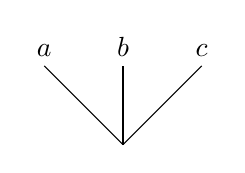
\begin{tikzpicture}
\draw (1,0) -- (0,1) node[above]{$a$} ;
\draw (1,0) -- (1,1) node[above]{$b$} ;
\draw (1,0) -- (2,1) node[above]{$c$} ;
\end{tikzpicture}
\end{center}
Of course, the source of such a map is the source of the first leave and the target is the target of the last leave. The identity maps are represented by the empty trees and the composition consists in joining the roots.
\end{itemize}
\end{defin}

One can repeat the process several times: $F^kC$ is the category with the same objects as $C$ and, as morphisms, the trees of heigh $k$ with maps of $C$ as leaves, which can be composed. The composition consists in joining the roots.\\

There is an obvious functor $\phi$ from $FC$ to $C$: it sends an object to itself ($Obj(FC)=Obj(C)$), and a tree (ie a morphism) to the composition of its leaves (in the previous tree picture, it sends the tree to $a \circ b \circ c$). Define also the obvious functor $:C \rightarrow FC$ which sends an object to itself and a morphism $a$ to the corresponding generator in $FC$, ie:
\begin{center}
\begin{tikzpicture}
\draw (0,0) -- (0,1) node[above]{$a$} ;
\end{tikzpicture}
\end{center}  


Similarly, there are natural functors between $F^2C$ and $FC$; one functor from $F2C$ to $F^2C$ and two functors in the opposite sense:
\begin{itemize}
\item $\phi F: F^2C \rightarrow FC$ reduces the branches between the height 1 and 2, ie:
\begin{center}
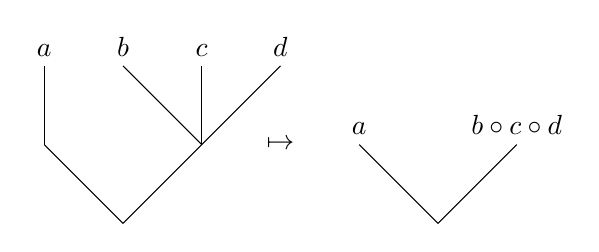
\begin{tikzpicture}
\draw (1,0) -- (0,1) ;
\draw (0,1) -- (0,2) node[above]{$a$} ;
\draw (1,0) -- (2,1) ;
\draw (2,1) -- (1,2) node[above]{$b$} ;
\draw (2,1) -- (2,2) node[above]{$c$} ;
\draw (2,1) -- (3,2) node[above]{$d$} ;

\draw (3,1) node{$\mapsto$};

\draw (5,0) -- (4,1) node[above]{$a$} ; 
\draw (5,0) -- (6,1) node[above]{$b \circ c \circ d$} ;
 
\end{tikzpicture}
\end{center}  
\item $F\phi : F^2C \rightarrow FC$ reduces the branches between the height 0 and 1, ie:

\begin{center}
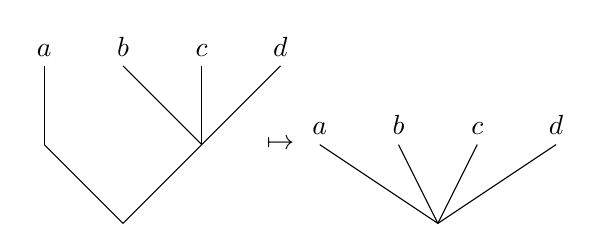
\begin{tikzpicture}
\draw (1,0) -- (0,1) ;
\draw (0,1) -- (0,2) node[above]{$a$} ;
\draw (1,0) -- (2,1) ;
\draw (2,1) -- (1,2) node[above]{$b$} ;
\draw (2,1) -- (2,2) node[above]{$c$} ;
\draw (2,1) -- (3,2) node[above]{$d$} ;

\draw (3,1) node{$\mapsto$};

\draw (5,0) -- (3.5,1) node[above]{$a$} ; 
\draw (5,0) -- (4.5,1) node[above]{$b$} ;
\draw (5,0) -- (5.5,1) node[above]{$c$} ;
\draw (5,0) -- (6.5,1) node[above]{$d$} ;
 
\end{tikzpicture}
\end{center}

\item Define also $\psi :: FC \rightarrow F^2C$:
%\begin{comment}
\begin{center}
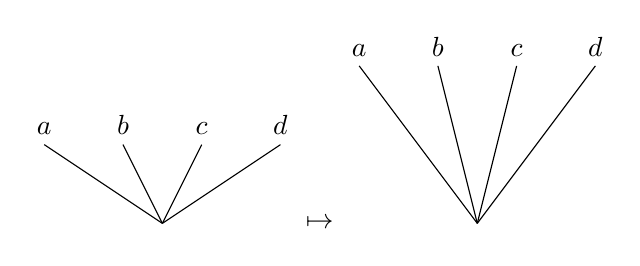
\begin{tikzpicture}
\draw (1.5,0) -- (0,1) node[above]{$a$} ; 
\draw (1.5,0) -- (1,1) node[above]{$b$} ;
\draw (1.5,0) -- (2,1) node[above]{$c$} ;
\draw (1.5,0) -- (3,1) node[above]{$d$} ;

\draw (3.5,0) node{$\mapsto$};

\draw (5.5,0) -- (4,2) node[above]{$a$} ; 
\draw (5.5,0) -- (5,2) node[above]{$b$} ;
\draw (5.5,0) -- (6,2) node[above]{$c$} ;
\draw (5.5,0) -- (7,2) node[above]{$d$} ;
\end{tikzpicture}
\end{center}
%\end{comment}
\end{itemize}

One notices for instance that $(F \phi) \psi=(F \phi) \psi$. One can also continue the process to higher order of free category; one then define in the same way $n$ functors from $F^n C$ to $F^{n-1} C$ and $n$ functors 

\begin{prop}
$(F^{k+1}C)_k$ together with the functors defined above is a simplicial category.
\end{prop} 

Furthermore this new category has the same homotopy type as $C$ (if we consider as a constant simplicial category

\begin{prop}
$(F^{k+1}C)_k \rightarrow C$ (functor unduced by the reduction of the trees) is a weak equivalence of categories (that means that it induces weak equivalences on the simplicial morphisms sets).
\end{prop} 

\begin{proof}[Sketch of the proof.]
Every tree of height $k$ is equivalent (in the homotopy sense) to the tree of same height and with only one leave which is the composition of the leaves.
\end{proof}

\subsubsection{The localization: definitions and first properties}

Along those lines, the morphisms of the localized categories $C[w^{-1}]$ are the tree of height $1$ such that its leaves are a succession of maps of $C$ and of $W$ (quotiented through an equivalence relation). The underlying idea of the standard simplicial localization is to look at the localization of $F^{k} C$ by $F^{k} W$.\\

Then, with few changes in the way of thinking with the respect to what we have in the previous sub-part, one can define: 

\begin{defin}
The (standard) simplicial localization of $(C,W)$ is the simplicial category $L(C,W)$ defined by:
\begin{equation}
L(C,W)_n=F^{n+1}C[(F^{n+1}W)^{-1}]
\end{equation}
\end{defin}

The homotopy groups of this localization is expected to encode the higher homotopy data data of $C$ with respect to $W$. Actually the homotopy relations are basically generated by the relation of two trees which have the same dimension and can be constructed from one same bigger tree. In dimension $0$, it gives the relation: 

\begin{prop}
$\pi_0 (LC(X,Y))=C[W^{-1}](X,Y)$
\end{prop}

\subsubsection{Generalization to simplicial categories}

One can generalise the notion of standard simplicial localization to simplicial categories.

\begin{defin}
If $A$ is a simplicial category, and $V$ a simplicial subcategory. The standard simplicial localization of $A$ with respect to $V$ is the simplicial category:
\begin{equation}
L(A,V)=diag(F^{*+1}A[(F^{*+1}V)^{-1}])
\end{equation} 
\end{defin}

We have something which is close of the old localization of an ordinary category if we take the path-components:
\begin{prop}
$\pi_0 (LB) =(\pi_0 B)[(im \pi_0 V)^{-1}]$
\end{prop}

Finally, let's see one lemma which can be useful:

\begin{lemma}[{\cite[6.3]{dksimplicial}}]
Let $A$ and $B$ two simplicial $C$-categories, $U$ a simplicial subcategory of $A$ and $V$ a simplicial subcategory of $B$, $S: A \rightarrow B$ a functor such that $S(U) \subset V$, and such that $S: A \rightarrow B$ and $S: U \rightarrow V$ are weak equivalence. Then the induced map $LA \rightarrow LB$ is a weak equivalence.
\end{lemma}

The demonstration of this last lemma is more complicated. One needs some machinery, as for instance a model structure on the category of the simplicial categories with the same objects as $C$ (this last category is not small).


\subsection{Hammock localization}

\subsubsection{Definition and first properties}
Let $C$ be a (small) category an $W$ a subcategory. Let's define the simplicial set $L^H (C,W)(X,Y)$ (or shortly $L^H C(X,Y)$); the $k$-simplices are the "reduced hammocks" of width $k$ and any length between $X$ and $Y$:

\[
\xymatrix{& {C_{0,0}} \ar@{-}[r] \ar[d] & {C_{0,1}} \ar[d] \ar@{--}[r] & {C_{0,n-1}} \ar@{-}[d] \ar@{-}[ddr] \\
& {C_{1,0}} \ar@{-}[r] \ar[d] & {C_{1,1}} \ar@{-->}[ddd] \ar@{--}[r] & {C_{1,n-1}} \ar@{-->}[ddd] \ar@{-}[dr] \\
X \ar@{-}[uur] \ar@{-}[ur] \ar@{--}[r] \ar@{-}[ddr] & {C_{2,0}} \ar@{-->}[dd] &&& {Y} \\
                                                                             \\
& {C_{k,0}} \ar@{-}[r] & {C_{k,1}} \ar@{--}[r] & {C_{k,n-1}} \ar@{-}[uur]}
\]

such that:
\begin{enumerate}
\item $n$, the length is $\geq 0$ (if $n=0$, the hammock consists in $k$-times the same morphism from $X$ to $Y$).
\item all vertical maps are in $W$.
\item in each column, all maps go to the same direction and if they go to the left, then they are in $W$.
\item the maps in adjacent columns go in different directions.
\item no column contains only identity maps.
\end{enumerate}

The $i^{th}$ face map $d_i$ consists in omitting the $i^{th}$ row. The $j^{th}$ degeneracy map consists in repeating the $j^{th}$ row. If the resulting hammock is not reduced (it can happen after the application of a face map), then one applies a reduction process:
\begin{enumerate}
\item if a column contains only identity maps, then one omits it.
\item one composes two adjacent columns whenever they go in the same direction
\end{enumerate}

Furthermore, there exists a distinguished vertices $id \in L^HC(X,X)$; if $X,Y$ and $Z$ are object of $C$, then one can also composition law $L^HC(X,Y) \times L^HC(Y,Z) \rightarrow L^H C(X,Z)$ which consists in, in each dimension, compose the hammocks and then reduce the resulting hammock. Then:

\begin{prop}
$L^H (C,W)$ is a simplicial category.
\end{prop}

The morphisms from $X$ to $Y$ of the localized category $C[W^{-1}]$ are the strings of successive arrows (i.e the elements of $L^HC(X,Y)_0$) quotiented by an equivalence relation. This equivalence is generated by the relation I call $\Re$; if $f,g \in L^HC(X,Y)_0$ then $ f \Re g$ if and only if:

\begin{center}
$\exists h \in L^H C(X,Y)_1 , d_0 (h)=f , d_1 (h)=g$
\end{center}

This just means:

\begin{prop}
For two objects $X,Y \in C$, then:
\begin{equation}
\pi_0 (L^H C(X,Y))=C[W^{-1}](X,Y)
\end{equation}
\end{prop}

Therefore, the underlying idea of the hammock localization is to study in a simplicial set the homotopy of string of arrows. Applying the equivalence gives us the usual localization, but makes us loose the higher homotopy data. The hammock localization is the good object to study this higher homotopy data.


\subsubsection{Generalisation to simplicial categories and link with the standard simplicial localization}

One can generalize the hammock localization to simplicial categories; if $B$ is a simplicial category and $V$ a simplicial subcategory (i.e a subcategory of $B$ together with inclusions of simplicial sets $V(X,Y) \rightarrow B(X,Y)$ which commute with the definition of identity and the composition):
\begin{enumerate}
\item $L^H(B,V)$ is an obviously defined bisimplicial category
\item the hammock localization of $B$ with respect to $V$ is $diag L^H(B,V)$
\end{enumerate}

\begin{rmk}
In the above description, one can equivalently use the formalism of simplicial objects over the category of simplicial (small) categories or of bisimplicial enriched categories;
\end{rmk}

There is an important lemma which comes with the description of the hammock of a simplicial category:

\begin{lemma}[{\cite[2.4]{dkcomputing}}]
If $A, B \in sC-cat$ (with the same set objects; see the introduction), and $U \subset A$, $V \subset B$ are simplicial subcategories, if $S : A \rightarrow B$ is a morphism in $sC-cat$ such that $S(U) \subset V$, and if $S:A \rightarrow B$ and $S: U \rightarrow V$ are weak equivalences (of simplicial $C$-categories), then it induces a weak equivalence of $C$-simplicial categories $diag L^H A \rightarrow diag L^H B$
\end{lemma}

This lemma is hard to prove. However, it is the main key for the next proposition:

\begin{prop}
If $C$ is a category and $W$ a subcategory (ordinary categories), then the natural functors:
\begin{equation}
L^H C \leftarrow diag L^H F^{*+1} \rightarrow F^{*+1} [(F^{*+1}W)^{-1}]
\end{equation}
are weak homotopy equivalences (in $sC-cat$).
\end{prop}

\begin{proof}[Ideas in the proof]
We don't make the proof but give its ingredients:
\begin{itemize}
\item the diagonal argument of bisimplicial sets
\item the homotopy lemma just above
\item the comparison lemma: if a category (ordinary) $D$ is freely generated by subcategories $E$ and $W$, then $L^H C \rightarrow C[W^{-1}]$ is a weak equivalence.
\end{itemize}
\end{proof}

So, we have make the link between the standard simplicial localization and the hammock localization. They are homotopy equivalent. Then one uses more the hammock localization as its definition is simpler and because it is simpler to work with it as we will see.

\subsubsection{The $II$-indexing category and hammock graphs}

The $II$ category is defined by:
\begin{enumerate}
\item its objects are the pairs $(S,T)$ of ordered subsets of $\mathbb{N}^*$ ($\mathbb{N}-\{0\}$) such that $S \cup T= \{1,...,|S \cup T|\}$.
\item the morphisms $(S,T) \rightarrow (S',T')$ are the order preserving maps $f: S \cup T \rightarrow S' \cup T'$ such that $f(S) \subseteq S'$ and $f(T) \subseteq T'$
\end{enumerate}

Let $C$ be a category and $W$ a subcategory (ordinary categories).

\begin{defin}
\begin{enumerate}
\item The category of $C$-graphs is defined by:
\begin{enumerate}
\item A $C$-graph is a graph (with directed edges i.e arrows) which set of points is $Obj(C)$.
\item A morphism $G_1 \rightarrow G_2$ of $C$-graph is the data of maps $G_1(X,Y) \rightarrow G_2(X,Y)$ for all $X$ and $Y$, objects of $C$, and where $G_1(X,Y)$ is the set of arrows from $X$ to $Y$ in $G_1$ (idem for $G_2$).
\end{enumerate}
\item the category of $C$-graphs corresponds to the category of $C$-simplicial categories but without the identity mapas and compositions. Indeed, one has the forgetful functor $C-cat \rightarrow C-graph$.
\item A simplicial $C$-graph is a simplicial object over the category of $C$-graph (or equivalently a $C$-graph with simplicial sets of arrows).
\item One has also the forgetful functor $sC-cat \rightarrow sC-graph$.
\item Weak equivalences between simplicial $C$-graphs are just morphisms of simplicial graphs which induce weak homotopy equivalences on the simplicial mapping spaces of arrows between two objects of $C$. This definition is the analogue to the definition of weak equivalence between simplicial $C$-categories.  
\end{enumerate}
\end{defin}

We can define a natural functor $\lambda C : II \rightarrow sC-graph$:
\begin{itemize}
\item An element of $II$ is equivalent to a word made with the letters $C$ and $W^{-1}$ in the way that transform, for example $(\{1,2\},\{3\})$ into $W^{-1} C C$.
\item From such a word, one made a simplicial $C$-graph describe by:
\begin{enumerate}
\item The arrows from $X$ to $Y$ (objects of $C$) are the unreduced hammocks:
\item the length of the hammocks is the length of the word we call $n$
\item The $i^{th}$ column is made of left-directed arrows of $C$ if the $(n+1-i)^{th}$ is $C$
\item The $i^{th}$ column is made of right-directed arrows of $W$ if the $(n+1-i)^{th}$ is $W^{-1}$  
\item These hammocks are organized in a simplicial set through the width as in $L^H C$.
\end{enumerate}
\item All of this is done functorially (because one can reduce parts of the hammocks and add column with the identity. For instance an injection in $II$ leads to the addition of identity maps in the corresponding $C$-graph). Therefore we have created a $II$-diagram in the category $sC-graph$
\item This diagram has a direct limit $lim \lambda C$
\end{itemize}


\begin{prop}
The reduction maps $r_{(S,T)} : \lambda C (S,T) \rightarrow L^H C$ (it is a morphism of the category $sC-graph$) induces a map $lim \lambda C \rightarrow L^H C$ which is a isomorphism.
\end{prop}

So we can see the hammock localization as a limit of graphs with simpler hammocks (of a definite type).

\begin{rmk}
This theory of $II$-diagrams is useful to prove the lemma introduced just above and non proved. However, we won't apply it to this purpose.
\end{rmk}

\subsubsection{Homotopy calculi of fractions}

Let $C$ be a category and $W$ a subcategory (ordinary categories).

\begin{defin}
$(C,W)$ is said to admit:
\begin{enumerate}
\item a homotopy calculus of (two-sided) fractions if, for every pairs $i,j >0$ the obvious maps in $sC-graph$ (adding a column with only identity):
\begin{equation}
W^{-1}C^{i+j}W^{-1} \rightarrow W^{-1}C^iW^{-1}C^jW^{-1}
\end{equation}
and
\begin{equation}
W^{-1}W^{i+j}W^{-1} \rightarrow W^{-1}W^i W^{-1} W^j W^{-1}
\end{equation}
are both weak equivalences (we consider the words as graph as seen just before).
\item a homotopy calculus of left fractions if, for every pairs $i,j >0$ the obvious maps in $sC-graph$:
\begin{equation}
W^{-1}C^{i+j} \rightarrow W^{-1}C^iW^{-1}C^j
\end{equation}
and
\begin{equation}
W^{-1}W^{i+j} \rightarrow W^{-1}W^i W^{-1} W^j
\end{equation}
are both weak equivalences.
\item a homotopy calculus of right fractions is defined in an analogue way.
\end{enumerate}
\end{defin}

The usefulness of the previous definition is due to the following proposition:

\begin{prop}[{\cite[6.2]{dkcomputing}}]
\begin{enumerate}
\item If $(C,W)$ admits a homotopy calculus of (two-sided) fractions, then the reduction maps
\begin{equation}
W^{-1}CW^{-1} \rightarrow L^H (C,W), W^{-1}WW^{-1} \rightarrow L^H (W,W)
\end{equation}
are weak equivalences.
\item one has the same kind of statement for the homotopy calculus of left or right fractions.
\end{enumerate}
\end{prop}

So, if the category admits a homotopy calculus of fractions, then the homotopy of its hammock localization is then much simpler to describe as we have only to consider hammocks of a certain shape.

\subsubsection{Case where the homotopy calculus is used}

\begin{defin}
$(C,W)$ admits a calculus of left fractions if:
\begin{enumerate}
\item For each diagram $\xymatrix{{X'} & X \ar[l]^u \ar[r]^f & Y}$ of $C$ with $u \in W$, there exists in $C$ a diagram $\xymatrix{{X'} \ar[r]^{f'} & {Y'}  & Y \ar[l]_v}$ with $v \in W$ and such that $v \circ f = f' \circ u$
\item If $f,g : X \rightarrow Y$ are morphisms of $C$ and $u :X' \rightarrow X$ is in $W$, and they are such that $f \circ u = g \circ u$, then there exists $v \in W$ such that $v \circ f= v \circ g$.
\end{enumerate} 
\end{defin}

Note that if $(C,W)$ admits a calculus of left fractions and if it is such that:
\begin{center}
if $f,g$ are morphisms of $C$ such that one can define $f \circ g$, and if two of the three morphisms $f$, $g$, and $f \circ g$ are in $W$, then the third is in $W$ 
\end{center}
then $(W,W)$ also admits a calculus of left fractions.\\


We have two important results about the calculus of left fractions:

\begin{prop}
If $(C,W)$ and $(W,W)$ admit a calculus of left fraction, then $(C,W)$ admits a homotopy calculus of left fraction.
\end{prop}

\begin{prop}
If $(C,W)$ and $(W,W)$ admit a calculus of left fraction, then the natural map:
\begin{equation}
L^H C \rightarrow \pi_0 L^H C = C[W^{-1}]
\end{equation}
is a weak equivalence of simplicial categories.
\end{prop}

Now, a final proposition which makes the hammock localization very useful in the frame of model category; here $M$ is a model category, $W$ refers to the weak equivalences, $M^c$ to the cofibrant subcategory, $M^f$ to the fibrant subcategory and $M^{cf}$ to the fibrant-cofibrant subcategory.

\begin{prop}
The pairs $(M,W)$, $(M^{c},W^{c})$, $(M^{f},W^{f})$ and $(M^{cf},W^{cf})$ admit homotopy calculi of two-sided fractions.
\end{prop}

\section{Homotopy simplicial category and conclusion}

We won't prove the following theorem which is the conclusion of our discussion:
\begin{thm}[{\cite[Thm. 4.4]{dkfunction}}]
Let $M$ be a model category. For any two objects $X,Y$ of $M$, if $X^*$ is a cosimplicial resolution of $X$ and $Y_*$ is a simplicial resolution of $Y$, then the simplicial sets $diag M(X^*,Y_*)$ and $L^H(X,Y)$ have the same homotopy type.
\end{thm}

\section{Complements to Chapter 2}

\subsection{Bisimplicial set}

\begin{defin}
A bisimplicial set is equivalently:
\begin{enumerate}
\item A simplicial object over the category $sSet$
\item A functor $(\Delta \times \Delta)^{op} \rightarrow Set$
\item A functor $\Delta^{op} \times \Delta^{op} \rightarrow Set$
\item A family of sets $(X_{n,m})_{(n,m) \in \mathbb{N}^2}$ together with two types of face maps and degeneracies such that the two simplicial structures commute.
\end{enumerate}
\end{defin}


The diagonal of a bisimplicial set is the obvious simplicial set made with the sets $X_{n,n}$, the face maps $X(d_i,d_i)$ and the degeneracies $X(s_j,s_j).$

\begin{comment}
\subsection{Auto equivalenc monoid}

\begin{defin}
A simplicial monoid is a simplicial obect in the category $Mon$ of monoids.
\end{defin}

\begin{defin}
Let $M$ be a model category with $W$ the subcategory of weak equivalences. Let $X$ an object of $M$. Then, the homotopy automorphisms complex $haut_{L^HM}X$ is the simplicial submonoid of $L^HM(X,X)$ which corresponds to the components which are invertible in $\pi_0 L^HM(X,X)$. In other words,
\begin{equation}
\forall n, haut_{L^HM}X_n=.....
\end{equation}
\end{defin}
\end{comment}

%\input{Quasicategories.tex}
%\input{Segal.tex}
%\chapter{Simplicial Presheaves}

The goal of this chapter is to explain the transition from the classical theory of stacks to the homotopical one. The main reference is \cite{hollander}. This chapter is organized as follows:
\begin{enumerate}
\item an introductory section about the classical theory of stacks, with some example;
\item the model structure on presheaves in groupoids and the equivalence;
\item the model structure on simplicial presheaves;
\item higher stacks and examples.
\end{enumerate}

\begin{flushright}
Mauro Porta
\end{flushright}

\section{Fibered Categories and Stacks}

We will assume some familiarity with Grothendieck topologies. I strongly recommend the book of MacLane and Moerdijk \cite[Ch. III]{sheaves} for a clear exposition of this theory. A neat treatment can be also found in the article \cite[Ch. II]{vistoli}.

\subsection{Fibered Categories}

\subsubsection*{Definitions and generalities}

Our exposition will follow \cite[Ch. III]{vistoli}, with some integration from \cite[Exposé VI]{sga1}. I strongly recommend the reader to think to fiber bundle (vector bundle if he prefers) while reading these notes.

For the whole exposition $\mathcal C$ will denote a fixed category.

\begin{notation}
If $\mathcal C$ is a category and $U \in \Ob(\mathcal C)$ is an object in $\mathcal C$, we will denote by $\kappa(U)$ the subcategory of $\mathcal C$ having $U$ as unique object and $\mathrm{id}_U$ as unique morphism, i.e. $\kappa(U)$ is the unique morphism $\Delta^0 \to \mathcal C$ defined by $* \mapsto U$.
\end{notation}

\begin{defin}
Let $p \colon \mathcal F \to \mathcal C$ be a category over $\mathcal C$ and let $U \in \Ob(\mathcal C)$. We define the fiber of $\mathcal F$ over $U$ as the subcategory of $\mathcal F$ mapping to $\kappa(U)$ via $p$. We will denote the fiber of $\mathcal F$ over $U$ as $\mathcal F_U$.
\end{defin}

\begin{rmk}
If $p \colon \mathcal F \to \mathcal C$ is a category over $\mathcal C$ and $U \in \Ob(\mathcal C)$, then $\mathcal F_U$ can be clearly described as the pullback (computed in $\Cat$):
\[
\xymatrix{
\mathcal F_U \ar[d] \ar[r] & \mathcal F \ar[d]^p \\ \kappa(U) \ar[r] & \mathcal C
}
\]
\end{rmk}

\begin{defin}
Let $\mathcal C$ be a category and let $p_\mathcal{F} \colon \mathcal F \to \mathcal C$ be a category over $\mathcal C$. An arrow $\phi \colon \xi \to \eta$ in $\mathcal F$ is said to be \emph{cartesian} if for every other arrow $\psi \colon \zeta \to \eta$ and any arrow $h \colon p_\mathcal{F} \zeta \to p_{\mathcal F} \xi$ in $\mathcal C$ such that $p_{\mathcal F} \phi \circ h = p_{\mathcal F} \psi$ there exists a unique arrow $\theta \colon \zeta \to \xi$ with $p_{\mathcal F} \theta = h$ and $\phi \circ \theta = \psi$.
\end{defin}

The following lemma contains some trivial but useful properties:

\begin{lemma} \label{lemma cartesian arrows}
Let $p \colon \mathcal F \to \mathcal C$ be a category over $\mathcal C$. Then:
\begin{enumerate}
\item the composition of two cartesian arrows is still cartesian;
\item if $\phi \colon \xi \to \eta$ is a cartesian arrow lying over $\mathrm{id}_{p(\eta)}$, then $\phi$ is an isomorphism;
\item every isomorphism in $\mathcal C$ is cartesian over its image.
\end{enumerate}
\end{lemma}

\begin{defin}
Let $p_{\mathcal F} \colon \mathcal F \to \mathcal C$ be a category over $\mathcal C$. We say that $\mathcal F$ is fibered over $\mathcal C$ if for every arrow $f \colon y \to x$ in $\mathcal C$ and any object $\eta \in \Ob(\mathcal F)$ such that $p_{\mathcal F}(\eta) = x$ there is a cartesian arrow $\phi \colon \xi \to \eta$ lying over $f$.
\end{defin}

\begin{eg} \label{eg cartesian serre fibration}
Consider a (Serre) fibration $p \colon X \to Y$ in $\cghaus$. Applying the fundamental groupoid functor $\Pi \colon \cghaus \to \grpd$ we get a functor $\Pi(p) \colon \Pi(X) \to \Pi(Y)$, and we claim that this functor defines a fibered category. In fact, choose an object $\eta \in \Pi(X)$, set $x = \Pi(p)(\eta)$. For every arrow $[\gamma] \colon y \to x$, represented by a continuous path
\[
\gamma \colon I = [0,1] \to Y
\]
introduce $\overline{\gamma} \colon I \to Y$, $\overline{\gamma}(t) = \gamma(1-t)$; since $p$ is a fibration we can lift $\overline{\gamma}$ to a path $[0,1] \to X$ sending $0$ to $\eta$. The lifting is unique up-to-homotopy, hence we obtain (taking again the inverse) an arrow
\[
[\phi] \colon \xi \to \eta
\]
mapping via $\Pi(p)$ to $[\gamma]$. Since $[\phi]$ is an isomorphism, it is cartesian (Lemma \ref{lemma cartesian arrows}), and so the assertion is proved.
\end{eg}

A fibered category has a property of homogeneity of fibers, as we are going to prove. Let's fix some notation. If $p \colon \mathcal F \to \mathcal C$ is a fibered category and $f \colon V \to U$ is an arrow in $\mathcal C$, denote by
\[
(\mathcal F \downarrow \mathcal F_U)_f
\]
the full subcategory of $(\mathcal F \downarrow \mathcal F_U)_f$ consisting of arrows $\phi$ such that $p(\phi) = f \circ g$ for some $g$ in $\mathcal C$.

\begin{lemma} \label{lemma homogeneity fibers}
Let $p \colon \mathcal F \to \mathcal C$ be a fibered category. For every arrow $f \colon V \to U$ in $\mathcal C$, there exists a functor
\[
\Phi_f \colon \mathcal F_U \to \mathcal (\mathcal F \downarrow \mathcal F_U)_f
\]
sending an object $\eta \in \Ob(\mathcal F_U)$ to a \emph{cartesian} arrow $\phi \colon \xi \to \eta$, with $\xi \in \Ob(\mathcal F_V)$.
is a cartesian arrow.
\end{lemma}

\begin{proof}
Consider the second projection functor:
\[
\Psi_f \colon (\mathcal F \downarrow \mathcal F_U)_f \to \mathcal F_U
\]
For each $\eta \in \Ob(\mathcal F_U)$ choose a cartesian arrow $\phi \colon \xi \to \eta$ lying over $f$. Then the pair $(\phi, \mathrm{id}_\eta)$ is a universal arrow from $\Psi_f$ to $\eta$.\footnote{This is the very definition of cartesian arrow, but remember also that all the arrows in $\mathcal F_U$ maps to the identity of $U$ via $p$.} It follows from the standard characterization of adjunctions (cfr. \cite[Theorem IV.1.2.(iv)]{cwm} that $\Psi_f$ has a right adjoint
\[
\Phi_f \colon \mathcal F_U \to (\mathcal F_V \downarrow \mathcal F_U)
\]
\end{proof}

Denote by $(\mathcal F_V \downarrow \mathcal F_U)_f$ the full subcategory of $(\mathcal F_V \downarrow \mathcal F_U)_f$ of arrows mapping to $f$ via $p$. Let
\[
\mathbf d \colon (\mathcal F_V \downarrow \mathcal F_U)_f \to \mathcal F_V
\]
the projection on the first component. Then, consider the functor $f^*$ defined as
\[
f^* := \mathbf d \circ \Phi_f \colon \mathcal F_U \to \mathcal F_V
\]
In this construction we are hiding the axiom of choice. We know from \cite[Theorem IV.1.2.(iv)]{cwm} that to construct the adjoint $f^*$ one has only to choose universal arrows for every object in $\mathcal F_U$. If we make this choice for every arrow $f \colon V \to U$ we obtain what is traditionally called a \emph{cleavage}:

\begin{defin}
A \emph{cleavage} of a fibered category $p \colon \mathcal F \to \mathcal C$ consists of a class $K$ of cartesian arrows in $\mathcal F$ such that for each arrow $f \colon U \to V$ in $\mathcal C$ and each object $\eta$ in $\mathcal F_V$ there exists a unique arrow in $K$ with target $\eta$ mapping to $f$ via $p$.
\end{defin}

\begin{lemma} \label{lemma pseudo functor 1}
Let $p \colon \mathcal F \to \mathcal C$ be a fibered category with cleavage $K$. Then
\begin{enumerate}
\item for each object $U \in \Ob(\mathcal C)$ there is an isomorphism
\[
\varepsilon_U \colon \mathrm{id}_U^* \to \mathrm{Id}_{\mathcal F_U}
\]

\item for each pair of composable arrows $f \colon V \to U$ and $g \colon W \to V$ in $\mathcal C$ there is a natural isomorphism
\[
\alpha_{f,g} \colon g^* f^* \to (fg)^*
\]

\item for each arrow $f \colon V \to U$ strict equalities
\[
\alpha_{\mathrm{id}_V,f} = \varepsilon_V f^*, \qquad \alpha_{f,\mathrm{id}_U} = f^* \varepsilon_U
\]

\item for each triple of arrows
\[
\xymatrix{ T \ar[r]^h & W \ar[r]^g & V \ar[r]^f & U }
\]
a diagram (strictly) commutative
\[
\xymatrix{
h^* g^* f^* \ar[d]_{h^* \alpha_{h,g}} \ar[r]^{\alpha_{h,g} f^*} & (gh)^* f^* \ar[d]^{\alpha_{gh,f}} \\ h^*(fg)^* \ar[r]^{\alpha_{h,fg}} & (fgh)^*
}
\]
\end{enumerate}
\end{lemma}

\begin{proof}
The existence of the natural transformations $\varepsilon_U$ and $\alpha_{f,g}$ is a trivial consequence of the uniqueness of the uniqueness up-to-natural-isomorphism of the adjoint (thus for example we observe that $\Phi_{fg}$ and $\Phi_g \circ \Phi_f$ give right adjoints to $\Psi_{fg}$ in the notation of the proof of Lemma \ref{lemma homogeneity fibers}, so that we obtain $\widetilde{\alpha}_{f,g} \colon \Phi_{fg} \to \Phi_g \circ \Phi_f$, and applying $\mathbf d$ we get the desired $\alpha_{f,g}$). The other checks are still a consequence of the adjointness; the technical details can be found in \cite[Prop. 3.11]{vistoli}.
\end{proof}

Accordingly to the traditional definitions, Lemma \ref{lemma pseudo functor 1} says that we can associate to every fibered category $p \colon \mathcal F \to \mathcal C$ a pseudo-functor
\[
\mathcal C^{\mathrm{op}} \to \Cat
\]

Conversely, we can associate to every pseudo-functor a fibered category:

\begin{lemma} \label{lemma pseudo functor 2}
Given a pseudo-functor $\Phi \colon \mathcal C^{\mathrm{op}} \to \Cat$ there is a fibered category $p \colon \mathcal F \to \mathcal C$ such that $\mathcal F_U = \Phi(U)$.
\end{lemma}

\begin{proof}[Sketch of the proof.]
The idea is roughly speaking to mimic the construction of a vector bundle starting from local trivializations. Define a category $\mathcal F$ whose objects are
\[
\bigcup_{U \in \Ob(\mathcal C)} \Ob(\Phi(U))
\]
If $(U,x)$ and $(V,y)$ are two objects in $\mathcal F$, define an arrow
\[
(U,x) \to (V,y)
\]
to be a pair $(f, \tau)$ where $f \colon U \to V$ is an arrow in $\mathcal C$ and $\tau \colon x \to \Phi(f)(y)$ is an arrow in $\Phi(U)$. The details for the construction can be found in \cite[Ch 3.1.3]{vistoli}.
\end{proof}

Finally the two constructions given in Lemma \ref{lemma pseudo functor 1} and \ref{lemma pseudo functor 2} are mutually inverse in a higher categorical sense.

\subsubsection*{Categories fibered in groupoids and in sets}

The equivalence between fibered categories and pseudo-functors with values in $\Cat$ suggests that fibered categories should be thought of as ``presheaves'' with values in $\Cat$. We will develop in detail this point of view later on. For the moment, we observe that it might be interesting to restrict the attention to categories whose fibers satisfy additional properties. Classically, the main interest is for categories fibered in groupoids.

\begin{defin}
A fibered category $p \colon \mathcal F \to \mathcal C$ is said to be \emph{fibered in groupoids} if each fiber $\mathcal F_U$ is a groupoid.
\end{defin}

An useful characterization is the one that follows:

\begin{prop} \label{prop fibered in groupoids}
A category $p \colon \mathcal F \to \mathcal C$ over $\mathcal C$ is fibered in groupoids if and only if:
\begin{enumerate}
\item every arrow in $\mathcal F$ is cartesian;
\item given any arrow $f \colon V \to U$ in $\mathcal C$ and any object $\eta \in \mathcal F_U$, there is an arrow $\phi \colon \xi \to \eta$ such that $p(\phi) = f$.
\end{enumerate}
\end{prop}

\begin{proof}
Straightforward (for details, see \cite[Proposition 3.22]{vistoli}.
\end{proof}

As a particular case, we have categories fibered in sets:

\begin{defin}
A fibered category $p \colon \mathcal F \to \mathcal C$ is said to be \emph{fibered in sets} if each fiber $\mathcal F_U$ is a set.
\end{defin}

\begin{prop} \label{prop fibered in sets}
A category $p \colon \mathcal F \to \mathcal C$ over $\mathcal C$ is fibered in sets if and only if for any object $\eta$ of $\mathcal F$ and any arrow $f \colon U \to p\eta$ of $\mathcal C$ there is a \emph{unique} arrow $\phi \colon \xi \to \eta$ of $\mathcal F$ with $p(\phi) = f$.
\end{prop}

\begin{proof}
Straighforward (see \cite[Proposition 3.25]{vistoli} for details).
\end{proof}

\begin{cor} \label{cor fibered in sets}
Let $p \colon \mathcal F \to \mathcal \mathcal C$ be a category fibered in sets. The associated pseudo-functor of Lemma \ref{lemma pseudo functor 1} is a functor that factorizes through $\Set \subset \Cat$.
\end{cor}

\begin{proof}
Proposition \ref{prop fibered in sets} implies that the isomorphisms $\alpha_{f,g}$ and $\varepsilon_U$ must be the identities. It follows that $\Phi$ is a functor; the factorization property descends from the very definition.
\end{proof}

\begin{rmk} \label{rmk fibered in sets}
Corollary \ref{cor fibered in sets} is saying that categories fibered in sets corresonds, under the equivalence sketched in Lemma \ref{lemma pseudo functor 1} and \ref{lemma pseudo functor 2}, to presheaves (of sets).
\end{rmk}

\subsubsection{The 2-category $(\Cat \downarrow \mathcal C)$}



\subsection{Descent Condition}

As we remarked at the end of previous section, fibered categories represents an extension of presheaves of sets. When the base category is endowed with a (Grothendieck) topology we can look for presheaves well-behaved with respect to the topology; classically, this leads to the notion of sheaf. In the more general context of categories fibered in groupoids, we will obtain stacks. The theoretical difficulty in this passage is contained in the fact that $\grpd$ is a 2-category, hence certain limits have to be understood in a 2-categorical sense. This suggests that we can, more generally, consider presheaves with values in a category carrying homotopical information; in that context, we will ask for limits and colimits to be understood in the homotopical sense (cfr. Section \ref{homotopy limits}).

\subsubsection*{Descent data}

There are several ways to define descent data and descent condition. We will follow the exposition given in \cite[Ch. 4]{vistoli}.

Let $(\mathcal C, J)$ be a site and let $p \colon \mathcal F \to \mathcal C$ be a category fibered in sets. For each object $U \in \Ob(\mathcal C)$ and each covering sieve $R$ on $U$, let
\begin{equation} \label{eq matching family}
\mathcal F(U)_R := \varprojlim_{V \to U \in R} \mathcal F_V
\end{equation}
It is well-known that this gives a description of the compatible families of objects with respect to the sieve $R$. A presheaf $\mathcal F$ is a sheaf if and only if the natural morphism
\begin{equation} \label{eq sheaf condition}
\mathcal F_U \to \mathcal F(U)_R
\end{equation}
is an isomorphism. If we want to generalize this construction to the context of categories fibered in groupoids, we have to give the correct meaning to equation \eqref{eq matching family}, and we will have to substitute the isomorphism \eqref{eq sheaf condition} with an equivalence of categories. Let's begin with the following observation:

\begin{lemma} \label{lemma transition sheaf stack}
With the previous notations and denoting by $\mathcal F$ the functor (cfr. Lemma \ref{rmk fibered in sets}) associated to $p \colon \mathcal F \to \mathcal C$, we have an isomorphism
\[
\mathcal F(U)_R \simeq \Hom(R,\mathcal F)
\]
\end{lemma}

\begin{proof}
Let $f \colon V \to U$ be an arrow in $R$ and define
\[
\alpha_f \colon \mathrm{Nat}(R, \mathcal F) \to \mathcal F(V)
\]
by setting
\[
\alpha_f(\varphi) := \varphi_V(V \to U)
\]
This gives a cone over $\{\mathcal F(V \to U)\}_{V \to U \in R}$ and so we get a morphism
\[
\Hom(R,\mathcal F) \to \mathcal F(U)_R
\]
It is straighforward to check that this is a bijection (cfr. \cite[Prop. 2.39]{vistoli}).
\end{proof}

Motivated by Lemma \ref{lemma transition sheaf stack} we give the following definition:

\begin{defin}
Let $p \colon \mathcal F \to \mathcal C$ be a fibered category over a site $(\mathcal C,J)$. For every covering sieve $R$ over an object $U \in \Ob(\mathcal C)$, define the descent data of $\mathcal F$ with respect to $R$ to be
\[
\mathcal F(U)_R := \mathbf{Hom}_{\mathcal C}(R, \mathcal F)
\]
where $R$ is reviewed as a full subcategory of $(\mathcal C \downarrow U)$.
\end{defin}

Observe that we have a natural arrow
\begin{equation} \label{eq stack condition}
\mathcal F_U \to \mathcal F(U)_R
\end{equation}
corresponding via the adjunction to the natural morphism
\[
\mathcal F_U \times_{\mathcal C} R \to \mathcal F
\]

Others description are possible. See \cite[Ch. 4.1.2]{vistoli} for a detailed explanation.

\begin{defin}
Let $p \colon \mathcal F \to \mathcal C$ be a fibered category on a site $(\mathcal C,J)$. We will say that:
\begin{enumerate}
\item $\mathcal F$ is a \emph{prestack} over $\mathcal C$ if for every covering sieve the natural functor \eqref{eq stack condition} is fully faithful;
\item $\mathcal F$ is a \emph{stack} over $\mathcal C$ if for every covering sieve the natural functor \eqref{eq stack condition} is an equivalence of categories.
\end{enumerate}
\end{defin}

\begin{prop}
Let $(C,J)$ be a site and let $p \colon \mathcal F \to \mathcal C$ be a category fibered in sets. Then
\begin{enumerate}
\item $\mathcal F$ is a prestack if and only if it is a separated functor;
\item $F$ is a stack if and only if it is a sheaf.
\end{enumerate}
\end{prop}

\begin{proof}
This is an immediate consequence of Lemma \ref{lemma transition sheaf stack}.
\end{proof}

\subsection{Examples}

\subsubsection{Quasi-coherent sheaves}

\begin{lemma} \label{lemma fpqc topology}
For any scheme $X$ say that a collection $\{\varphi_i \colon U_i \to X\}_{i \in I}$ is a fpqc covering if each $\varphi_i$ is flat and quasi-compact and if the family of maps is jointly surjective. Then the fpqc covers satisfy the axioms for a pretopology.
\end{lemma}

\begin{proof}
We have to show that a fpqc morphism is stable under base change, but this is clear.
\end{proof}

\begin{defin}
Let $S$ be a scheme. The (big) fpqc site over $S$ is the category $\mathbf{Sch} / S$ endowed with the fpqc topology defined in Lemma \ref{lemma fpqc topology}.
\end{defin}

Fix a scheme $S$ and consider the (big) fpqc site over $S$, $(\mathbf{Sch}/S)_{\mathrm{fpqc}}$. Define a pseudo-functor
\[
\Phi \colon (\mathbf{Sch}/S)_{\mathrm{fpqc}}^{\mathrm{op}} \to \Cat
\]
on objects as
\[
\Phi(X) := \mathrm{QCoh}(X)
\]
the category of quasi-coherent $\mathcal O_X$-modules. To define the action on arrows, recall the following lemma:

\begin{lemma}
Let $f \colon X \to Y$ be a morphism of schemes. Then if $\mathcal G$ is a quasi-coherent module over $Y$, $f^* \mathcal G$ is a quasi-coherent module over $X$.
\end{lemma}

\begin{proof}
Immediate consequence of the exactness of $f^{-1}$ and the right-exactness of
\[
- \otimes_{\mathcal O_R} \mathcal F \colon \mathbf{Mod}_{\mathcal O_R} \to \mathbf{Mod}_{\mathcal O_R}
\]
where $\mathcal O_R$ is a sheaf of rings and $\mathcal F$ is a $\mathcal O_R$-module (the reader not at ease with Algebraic Geometry might would like to check on \cite[Prop. II.5.8.(a)]{hartshorne}).
\end{proof}

To check that we obtain a pseudo-functor we observe that $\mathrm{QCoh}(X)$ is a full subcategory of $\mathbf{Mod}_{\mathcal O_X}$ and that $f^*$ is defined also for the larger category.


The difference, is that the functor
\[
f^* \colon \mathbf{Mod}_{\mathcal O_Y} \to \mathbf{Mod}_{\mathcal O_X}
\]
has a right adjoint, namely
\[
f_* \colon \mathbf{Mod}_{\mathcal O_X} \to \mathbf{Mod}_{\mathcal O_Y}
\]

\begin{rmk}
Recall that in general $f_*$ doesn't induce a functor
\[
f_* \colon \mathrm{QCoh}(X) \to \mathrm{QCoh}(Y)
\]
For example it is not true that a skyscraper sheaf is quasi-coherent,\footnote{Observe that if $\widetilde{M}_x \ne 0$, then for each $y \in \overline\{x\}$ we have also $\widetilde{M}_y \ne 0$. This allows to construct a simple counter-example over a non-closed point.} at least without additional hypothesis on $f$ (e.g. quasi-compact and separated).
\end{rmk}

The adjointness allows to construct the required isomorphisms $\alpha_{f,g}$ and $\varepsilon_X$. For the details, see \cite[Ch. 3.2.1]{vistoli}. Let now
\[
\mathbf{QCoh}_S \to \mathbf{Sch}/S
\]
be the fibered category associated to $\Phi$ via the construction in Lemma \ref{lemma pseudo functor 2}. We can show:

\begin{thm}
$\mathbf{QCoh}_S \to \mathbf{Sch}/S$ is a stack.
\end{thm}

\begin{proof}
See \cite[Thm. 4.23]{vistoli}.
\end{proof}

\subsubsection{Elliptic curves}

The current goal is twofold: showing that stacks provide an useful enlargement of sheaves and construct an interesting example. More in detail, we want to show that if we want to deal with elliptic curves over a scheme, the na{\"i}f approach of taking isomorphism classes fails (we do not get back a sheaf); however, if we don't forget isomorphisms and we consider the category fibered in groupoids, we get a stack.

\begin{defin}
Let $S$ be a scheme. An elliptic curve over $S$ is a triple $(E,f,0)$ where
\begin{enumerate}
\item $f \colon E \to S$ is proper, smooth and of relative dimension $1$;
\item for every $s \in S$ the fiber $E_s$ is a geometrically connected curve of genus $1$;
\item $0 \colon S \to E$ is a section of $f$.
\end{enumerate}
\end{defin}

Consider the site $\mathbf{Sch}_{\mathrm{{\'e}t}}$. Define a presheaf
\[
\Phi \colon \mathbf{Sch}_{\mathrm{{\'e}t}} \to \Set
\]
sending a scheme $S$ to the set of isomorphism classes of elliptic curves over $S$. If $g \colon S' \to S$ is a morphism of scheme and $(E,f,0)$ is an elliptic curve over $S$ we construct an elliptic curve $(E',f',0')$ over $S'$ via the fiber product:
\[
\xymatrix{
E' = E \times_S S' \ar[d]^{f'} \ar[r] & E \ar[d]^f \\ S' \ar[r]^g & S
}
\]
From \cite[Prop. 3.3.16.(c)]{liu} we see that $f'$ is still proper; from \cite[Prop. 4.3.38]{liu} we see that $f' \colon E' \to S'$ is still a smooth morphism. Recall that in this case the relative dimension at a point $x$ is the rank of $\Omega^1_{E'/S'}$ at $x$; \cite[Prop. 1.8.(a)]{liu} shows then that $f' \colon E' \to S'$ is still of relative dimension $1$. The fibers of $f'$ are again geometrically connected because this property is stable under base change; finally, the genus is invariant under field extensions, and this is sufficient to conclude.

The functoriality of this construction shows that isomorphism classes of elliptic curves over $S$ are sent into isomorphism classes if elliptic curves over $S'$, hence we get a map
\[
g^* \colon \Phi(S) \to \Phi(S')
\]
It is straightforward to check that the so-defined $\Phi$ is a presheaf. We want to show that $\Phi$ cannot be a sheaf: let $S = \mathrm{Spec}(\mathbb F_3)$ and consider the elliptic curves
\begin{gather*}
C := \{(x,y) \in \mathbb A^2_{\mathbb F_3} \mid y^2 = x^3 - x - 1 \} \\
D := \{(x,y) \in \mathbb A^2_{\mathbb F_3} \mid y^3 = x^3 - x + 1 \}
\end{gather*}
They cannot be isomorphic because a simple direct check shows that $C$ doesn't have $\mathbb F_3$-rational points, while $D$ has $7$ $\mathbb F_3$-rational points. However, if $K$ is a finite field extension of $\mathbb F_3$ containing a square root of $1$, then
\[
\mathrm{Spec}(K) \to \mathrm{Spec}(\mathbb F_3)
\]
is an étale covering of $\mathrm{Spec}(\mathbb F_3)$, and $C_K$ is isomorphic to $D_K$. Therefore, the canonical map
\[
\xymatrix{
\Phi(\mathbb F_3) \ar[r] & \Phi(K) \ar@<.5ex>[r]^{\mathrm{id}} \ar@<-.5ex>[r]_{\mathrm{id}} & \Phi(K)
}
\]
is not injective; in particular $\Phi$ cannot be a sheaf. Under the identification constructed before, we can also say that $\Phi$ is not a stack.

The situation changes drastically if we don't take isomorphism classes of elliptic curves. Define
\[
\mathcal M_{\mathrm{ell}} \colon \mathbf{Sch}_{\mathrm{{\'e}t}} \to \grpd
\]
defined on objects sending a scheme $S$ into the category $\mathcal M_{\mathrm{ell}}(S)$ whose objects are elliptic curves over $S$ and whose morphisms are isomorphisms of elliptic curves. $\mathcal M_{\mathrm{ell}}$ is in fact a pseudo-functor: the construction $\alpha_{f,g}$ is, as usual, due to the universal property of the pull-back that we are using.\footnote{We are sloppy on these checks because in fact the $(\infty,1)$ viewpoint \emph{should} allow a \emph{complete} and \emph{formal} proof of these facts, using the property that maps obtained via a (standard categorical) universal property define always a contractible space.} 

We want to check 

\subsubsection{Quotients}

Stacks are well-suited to deal with quotients by group action. We will discuss in general this example, and we will specialize it to two different situation: an algebraic one, and a differentiable one.

\section{Model structure on presheaves in groupoids}

As we were suggesting, the difficulty that separates the notion of sheaf from that of stack is related to the fact that $\grpd$ carries a homotopical structure (see Theorem \ref{model structure on groupoids}). In this section we reformulate the notion of stack using the machinery of model categories developed in Chapter 1.


\subsection{Via the adjunction}

\subsection{Via Bousfield localization}

\section{Simplicial Presheaves}

\cite{jardinepresheaves}

\subsection{Injective Model Structure}

\subsection{Hypercovers}

\cite{hypercover}

\subsection{Characterization of fibrant objects}


\section{Higher Stacks}

\section{Complements to Chapter 3}

\subsection{Cartesian closedness of $\Cat$}

The main reference is \cite[Ch. VI]{sga1}.

\begin{lemma} \label{lemma internal hom adjunctions}
For each category $\mathcal C$ the functor $\mathbf{hom}(\mathcal C, -) \colon \Cat \to \Cat$ preserves the adjunctions.
\end{lemma}


\chapter{Differential graded categories}
\begin{flushright}
  Pieter Belmans
\end{flushright}

\section{Introduction}
The notion of triangulated category lies at the heart of homological algebra. This type of category is essential in the study of derived categories and stable homotopy categories of spectra. But there are some problems with this concept: the cone construction is not-functorial. Already in Verdier's PhD thesis there is the result that if the cones in a (countably) (co)complete triangulated category are functorial that category is necessarily semisimple abelian \cite[proposition II.1.2.13]{verdierphd}. As not every triangulated category is abelian \cite[exercise 1.4.5]{weibel} this is a problem\expandthis{why exactly is this a problem?}. To put it more bluntly:
\begin{quote}
  ``This `nonfunctoriality of a cone' is the first symptom that something is going wrong in the axioms of a triangulated category.''
\end{quote}
\begin{flushright}
  \cite[section IV.7]{gelfandmanin}
\end{flushright}
Another symptom is that certain theorems involving derived categories are ``weak'', in the sense that one might suspect them to hold in a more general context. By enriching the category before applying the constructions from homological algebra, we can retain enough information about the original category to solve some of the issues.

In a more abstract context: up to now we have seen that there are different models for~$(\infty,1)$\dash categories. The models we have discussed so far are quasicategories, relative categories using simplicial localisation, Segal categories and complete Segal spaces. These are all models for the general theory of~$(\infty,1)$\dash categories. One could restrict himself on the other hand to certain subclasses of~$(\infty,1)$\dash categories. An important example of this phenomenon are model categories, which provide a model for certain~$(\infty,1)$\dash categories that are both complete and cocomplete. Whether they can model \emph{all} complete and cocomplete~$(\infty,1)$\dash categories is not known. Another possible subclass of~$(\infty,1)$\dash categories is the one modelled using differential graded categories. They are so called ``linear'' models, in the same sense that homological algebra is a linear version of homotopical algebra.

Whereas topological or simplicial categories are categories enriched over topological spaces or simplicial sets, a differential graded category is a category enriched over (co)chain complexes of~$k$\dash modules, for~$k$ a commutative ring. So we restrict ourselves from~$\infty$\dash groupoids to so called abelian and fully strict~$\infty$\dash groupoids, these are exactly the~$\infty$\dash groupoids modelled by chain complexes.

The goal of this expos\'e is to
\begin{enumerate}
  \item introduce dg~categories;
  \item discuss the model category structures on the category of dg~categories;
  \item give some applications of this machinery;
  \item explain how to construct a dg~category from a~$(\infty,1)$\dash category.
\end{enumerate}

The main expository references for dg~categories are \cite{lnm2008,keller}. The results in this expos\'e are obtained in \cite{toen}. Other interesting papers are \cite{toen-vaquie}\expandthis.


\section{Differential graded categories}
From now on we fix a commutative ring~$k$. Every construction is relative to this base ring. Whenever the ring is required to be a field it will be specified. We moreover use cochain complexes, i.e.\ the degree of the differential is~$1$, but the exposition can be done completely the same using chain complexes and morphisms of degree~$-1$.

As already suggested, the definition of a dg~category is easy. We will freely use the language of enriched categories, but whenever a down-to-earth interpretation can be made it will be given.
\begin{definition}
  \label{definition:dg-category-enriched}
  A \emph{dg~category} is a category enriched over cochain complexes of~$k$\dash modules.
\end{definition}
A cochain complex can equivalently be considered as a dg~$k$\dash module: it is a graded~$k$\dash module equipped with a differential~$\dd$ of degree~$1$. The monoidal structure of~$k\textrm{-}\Mod$ implies that the composition in a dg~category~$\mathcal{C}$
\begin{equation}
  \Hom_{\mathcal{C}}(Y,Z)^\bullet\otimes_k\Hom_{\mathcal{C}}(X,Y)^\bullet\to\Hom_{\mathcal{C}}(X,Z)^\bullet
\end{equation}
is a morphism of dg~$k$\dash modules. Remark that the tensor product of graded~$k$\dash modules~$V^\bullet$ and~$W^\bullet$ is given by
\begin{equation}
  (V^\bullet\otimes_k W^\bullet)^n\coloneqq\bigoplus_{\mathclap{p+q=n}}V^p\otimes_k W^q.
\end{equation}

\expandthis{discuss dg modules}

\section{Model category structures on~$\dgCat_k$}
It is possible to put at least two different model category structures on~$\dgCat_k$: one with quasi-equivalences as weak equivalences, and the other with Morita morphisms as weak equivalences.

We start with the ``canonical'' model category structure, where the quasi-equivalences are inverted.
\begin{definition}
  Let~$f\colon\mathcal{C}\to\mathcal{D}$ be a morphism in~$\dgCat_k$, i.e.\ a dg~functor between dg~categories. It is said to be \emph{quasi-fully faithful} if for all~$X,Y\in\Ob(\mathcal{C})$ the map
  \begin{equation}
    f_{X,Y}\colon\Hom_{\mathcal{C}}(X,Y)^\bullet\to\Hom_{\mathcal{D}}(f(X),f(Y))^\bullet
  \end{equation}
  of cochain complexes is a quasi-isomorphism. It is said to be \emph{quasi-essentially surjective} if the induced functor
  \begin{equation}
    \HH^0(f)\colon\HH^0(\mathcal{C})\to\HH^0(\mathcal{D})
  \end{equation}
  on the level of ($k$\dash linear) categories is essentially surjective.
\end{definition}
These are versions of the two conditions necessary to define the equivalence of categories that are compatible with the enrichment, hence we can define the following.
\begin{definition}
  Let~$f\colon\mathcal{C}\to\mathcal{D}$ be a morphism in~$\dgCat_k$. It is said to be a \emph{quasi-equivalence} if it is both quasi-fully faithful and quasi-essentially surjective.
\end{definition}
We now introduce the fibrations in this model category structure.
\begin{definition}
  \label{definition:quasi-fibration}
  Let~$f\colon\mathcal{C}\to\mathcal{D}$ be a morphism in~$\dgCat_k$. It is said to be a \emph{quasi-fibration}\index{quasi-!fibration} if
  \begin{enumerate}
    \item for all~$X,Y\in\Ob(\mathcal{C})$ the map
      \begin{equation}
        f_{X,Y}\colon\Hom_{\mathcal{C}}(X,Y)^\bullet\to\Hom_{\mathcal{D}}(f(X),f(Y))^\bullet
      \end{equation}
      is a fibration in~$\Ch(k)$ for the projective model category structure on~$\Ch(k)$, i.e.\ is it an epimorphism in every degree;
    \item for all~$X\in\Ob(\mathcal{C})=\Ob(\HH^0(\mathcal{C}))$ and for all isomorphisms~$v\colon\HH^0(f)(X)\to Y$ in~$\HH^0(\mathcal{D})$ we can lift~$v$ to an isomorphism~$u\colon X\to Y$ in~$\HH^0(\mathcal{C})$ such that~$\HH^0(f)(u)=v$.
  \end{enumerate}
\end{definition}

\begin{theorem}[\cite{tabuada}]
  \label{theorem:quasi-equivalences-model-category-structure}
  If we take take the quasi-equivalences as weak equivalences, the quasi-fibrations as fibrations, and the dg~functors satisfying the right lifting property with respect to the trivial fibrations as cofibrations we obtain a model category structure on~$\dgCat_k$.
\end{theorem}

In the second model category structure we use a bigger class of weak equivalences, the same fibrations and therefore a smaller class of cofibrations. Its main uses are \expandthis{what is it good for?}
\begin{definition}
  Let~$\mathcal{C}$ be a dg~category. Its \emph{derived category of dg~$\mathcal{C}$\dash modules}~$\mathbf{D}\dgMod{\mathcal{C}}_k$ is the localisation of~$\dgMod{\mathcal{C}}_k$ with respect to the quasi-isomorphisms.
\end{definition}
Associated to a dg~functor~$f\colon\mathcal{C}\to\mathcal{D}$ is the restriction functor
\begin{equation}
  f^*\colon\dgMod{\mathcal{D}}_k\to\dgMod{\mathcal{C}}_k
\end{equation}
given by composition. This yields the following definition.
\begin{definition}
  Let~$f\colon\mathcal{C}\to\mathcal{D}$ be a morphism in~$\dgCat_k$. It is said to be a \emph{Morita morphism} if
  \begin{equation}
    \mathbf{D}f^*\colon\mathbf{D}\dgMod{\mathcal{D}}_k\to\mathbf{D}\dgMod{\mathcal{C}}_k
  \end{equation}
  is an equivalence of categories.
\end{definition}

\begin{theorem}[\cite{tabuada-2}]
  \label{theorem:morita-morphisms-model-category-structure}
  If we take take the Morita morphisms as weak equivalences, the quasi-fibrations as fibrations, and the dg~functors satisfying the right lifting property with respect to the trivial fibrations as cofibrations we obtain a model category structure on~$\dgCat_k$.
\end{theorem}

\section{Mapping spaces}

\section{Monoidal structure}

\section{Derived dg categories}

\section{$(\infty,1)$ and dg categories}


\appendix

%\chapter{Simplicial Sets}

It is a fact that Topology is absolutely central in Mathematics; this general framework developed in the first decades of the XXth century provides powerful techniques to handle problems in Analysis, Geometry, Algebra. Perhaps even more importantly, Topology gives a unifying point of view and shows how branches of Mathematics apparently unrelated, in reality share a deep connection. During a first approach, we have been taught to think about (point-set) topology as something axiomatizing the notion of ``being close''. This is a static vision of Topology; there is another one, concerning deformations and homotopies. ``Reduce to a simpler case'', this is one of the fundamental \emph{mantras} of Mathematics; in the topological context, where pathological examples abound, one of the most useful techniques is to deform the object of study into a nicer one, obviously preserving the properties we are interested in. More recently, certain mathematicians began to realize that deformations techniques can be successfully employed in several areas, for example in Algebraic Geometry. One of the goals of these notes is to convince the readers that the topological situation is universal with respect to deformation theories, as much as we think sets as universal with respect to (the most of the) Mathematics.

Simplicial sets were born as an attempt to minimize the structure needed in order to develop a homotopy theory, without changing the final result. In a sense, we can look at simplicial sets as a ``homotopical skeleton'' of topological spaces. The resulting theory is quite powerful, and it took the foundational position of topological spaces in all the questions concerning homotopy theory. In Chapter 1, for example, we show that it is always possible to construct \emph{meaningful} functors from any model category to the category of simplicial sets, taking the place of the hom-sets in classical category theory.

If this reduction process is convenient from a foundational and conceptual point of view, however, it surely adds more technicalities. Simple reasoning in topology can be impossible to literally translate in this new world; still, it is a good enough principle to think that every deep result in $\Top$ translates into an analogous statement for $\sset$. As a practical example, consider the definition of homotopy itself: in $\Top$ we have several different ways to define homotopy, and they are all more or less trivially equivalent. In $\sset$ the definitions can be easily translated; however, the proof of the equivalence requires more work. As general tool, the theory of anodyne extensions provides a way to skip many of these tedious details, at the price of a new set of standard arguments and tricks that one has to learn.

\section{The category $\SDelta$ and (co)simplicial objects}

\begin{notation}
For every $n \in \N$ let $\mathbf n$ be the category associated to the (unique) linearly ordered set with $n$ elements.
\end{notation}

\begin{defin}
Let $\SDelta$ be the full subcategory of $\Cat$ spanned by the categories $\mathbf n$ as $n$ varies in $\N$.
\end{defin}

\begin{rmk}
$\SDelta$ is thus the category whose objects are finite totally ordered sets and whose arrows are (weakly) increasing functions.
\end{rmk}

Let $\mathbf n, \mathbf m \in \SDelta$. We want an easy (= combinatorial) way to describe the hom-set
\[
\Hom_{\SDelta}(\mathbf n, \mathbf m)
\]
The idea is to look for elementary arrows. For example, if $\mathbf m = \mathbf{n+1}$ then we have exactly $n+1$ \emph{strictly} increasing arrows, namely $d^i \colon \mathbf n \to \mathbf{n+1}$ ($i \in \{0,1,\ldots,n+1\}$) defined by
\[
d^i(j) = \begin{cases} j & \text{if } j < i \\ j + 1 & \text{if } j \ge i \end{cases}
\]
We will call the maps $d^i$ the coface maps.

Similarly, we can construct $n+1$ arrows $s^i \colon \mathbf{n+1} \to \mathbf n$ by requiring that exactly two successive numbers have the same image:
\[
s^i(j) = \begin{cases} j & \text{if } j \le i \\ j - 1 & \text{if } j > i \end{cases}
\]
We will call the maps $s^i$ the codegeneracy maps.

The first basic result is that those arrows allows to completely describe all the arrows in $\SDelta$:

\begin{thm} \label{thm factorization epi-mono for Delta}
Let $f \colon \mathbf n \to \mathbf m$ be any arrow in $\SDelta$. Then there are uniquely determined maps $d,s \in \mathrm{Ar}(\SDelta)$ such that
\[
f = d \circ s
\]
where
\begin{equation} \label{eq increasing part}
d = d^{i_1} \circ \ldots \circ d^{i_s} \qquad 0 \le i_s \le \ldots \le i_1 \le m
\end{equation}
and
\begin{equation} \label{eq decreasing part}
s = s^{j_1} \circ \ldots \circ s^{j_r} \qquad 0 \le j_1 < \ldots < j_t < n
\end{equation}
\end{thm}

\begin{rmk}
Before starting the proof, let's observe that if $f \colon \mathbf n \to \mathbf m$ is injective (surjective) as map of sets, then it is monic (epi) in $\SDelta$. This is essentially obvious, and has as simple consequence the fact that any iterated composition of the face maps $d^i$ is monic.
\end{rmk}

\begin{proof}
Let $i_s < \ldots < i_1$ be the elements in $\mathbf m$ not in the image of $f$, and let $j_1 < \ldots < j_t$ be the elements in $\mathbf n$ such that $f(j) = f(j+1)$. Write also
\[
p = n -t = m - s
\]
We claim that with this choice of indexes, equations \eqref{eq increasing part} and \eqref{eq decreasing part} gives the desired factorization:
\[
\xymatrix{ \mathbf n \ar[r]^d & \mathbf p \ar[r]^s & \mathbf m }
\]
In fact, fix $k \in \{0,1,\ldots,n\}$. Assume that $j_h \le k < j_{h+1}$. Then necessarily $f(k)$ is the $(k-h)$-th element in $\mathbf m \setminus \{i_1,\ldots,i_s\}$; therefore
\[
f(k) = d(k-h) = d(s(k))
\]
The factorization is unique because if $f$ miss $i_s,\ldots,i_1$, then $f$ must factor through $d$, hence $f = d s'$, and since $d$ is mono, $s' = s$.
\end{proof}

Theorem \ref{thm factorization epi-mono for Delta} shows us that the collection of coface maps and codegeneracy maps generates all the arrows in $\SDelta$. We can describe their mutual relations by the so-called co-simplicial identities:

\begin{equation} \label{eq cosimplicial identities}
\begin{gathered}
d^j d^i = d^i d^{j-1} \quad \text{if } i < j \\
s^j s^i = s^i s^{j+1} \quad \text{if } i \le j \\
s^j d^i = \begin{cases} d^i s^{j-1} & \text{if } i < j \\
\text{id} & \text{if } i = j \text{ or } i = j + 1 \\
d^{i-1} s^j & \text{if } i > j+1 \end{cases}
\end{gathered}
\end{equation}

The proof does not give any deeper insight. The easiest way to convince yourself of those identities is to draw these maps of linearly ordered sets. We will skip on the details. The importance of the cosimplicial identities is that they completely describe the internal structure of $\SDelta$. This can be formalized as following:

\begin{thm} \label{thm presentation for Delta}
Let $\mathcal D$ be the graph whose objects are natural numbers and such that for each $n \in \N$ there are exactly $n+2$ arrows $\delta^i_n$ ($i \in \{0\,\ldots,n+1\}$) with source $n$ and target $n+1$, and exactly $n+1$ arrows $\sigma^i_n$ ($i \in \{0,\ldots,n\}$) with source $n$ and target $n-1$. Then $\SDelta$ is obtained as the quotient of the free category $F \mathcal D$ via the relations \eqref{eq cosimplicial identities}.
\end{thm}

\begin{proof}
We have to check the universal property of the quotient. Let $G \colon F \mathcal D \to \mathcal C$ be a functor such that the maps $G(\delta^i_n)$ and $G(\sigma^i_n)$ satisfy the cosimplicial identities. Then define $\overline{G} \colon \SDelta \to \mathcal C$ using the factorization epi-mono provided in Theorem \ref{thm factorization epi-mono for Delta}; the simplicial identities allows to check functoriality of this definition. Uniqueness is clear.
\end{proof}

\begin{rmk}
Previous theorem gives us a presentation for $\SDelta$.
\end{rmk}

\begin{defin} \label{def (co)simplicial objects}
Let $\mathcal C$ be any category. A cosimplicial object in $\mathcal C$ is a functor $F \colon \SDelta \to \mathcal C$; a simplicial object is $\mathcal C$ is a functor $F \colon \SDelta^\text{op} \to \mathcal C$.
\end{defin}

As consequence of Theorem \ref{thm presentation for Delta} we get immediately

\begin{cor}
Let $\mathcal C$ be any category. To give a cosimplicial object $A$ in $\mathcal C$, it is necessary and sufficient to give a sequence of objects $\{A^n\}_{n \in \N}$ together with coface operators $\partial^i \colon A^{n-1} \to A^n$ and codegeneracy operators $\sigma^i \colon A^{n+1} \to A^n$ ($i = 0,\ldots,n$) satisfying the cosimplicial identities
\begin{gather*}
\partial^j \partial^i = \partial^i \partial^{j-1} \quad \text{if } i < j \\
\sigma^j \sigma^i = \sigma^i \sigma^{j+1} \quad \text{if } i < j \\
\sigma^j \partial^i = \begin{cases}
\partial^i \sigma^{j-1} & \text{if } i < j \\
\mathrm{id} & \text{if } i = j \text{ or } i = j+1 \\
\partial^{i-1} \sigma^j & \text{if } i > j+1
\end{cases}
\end{gather*}
\end{cor}

\begin{cor}
Let $\mathcal C$ be any category. To give a simplicial object in $\mathcal C$ it is necessary and sufficient to give a sequence of objects $\{A_n\}_{n \in \N}$ together with face operators $\partial_i \colon A^{n+1} \to A^n$ and degeneracy operators $\sigma_i \colon A_{n-1} \to A_n$ ($i = 0, \ldots, n$) satisfying the simplicial identities
\begin{gather*}
\partial_i \partial_j = \partial_{j-1} \partial_i \quad \text{if } i < j \\
\sigma_i \sigma_j = \sigma_{j+1} \sigma_i \quad \text{if } i < j \\
\partial_i \sigma_j = \begin{cases} \sigma_{j-1} \partial_i & \text{if } i < j \\
\mathrm{id} & \text{if } i = j \text{ or } i = j+1 \\ \sigma_j \partial_{i-1} & \text{if } j > j+1 \end{cases}
\end{gather*}
\end{cor}

\begin{proof}
Just observe that these simplicial identities are exactly the dual of the cosimplicial ones.
\end{proof}

\section{Simplicial sets}

\subsection{Definitions and examples}

According to Definition \ref{def (co)simplicial objects}, a simplicial set is just a presheaf over $\SDelta$. We will denote this category by $\sset$. The reader should know that this abstract definition won't be of any help in understanding the rich theory of simplicial sets. However, it allows to develop quickly a large amount of theory.

\begin{defin}
Let $K \in \sset$. For each $n \in \N$, the set $K_n := K(\mathbf n)$ is called the set of $n$-simplices in $K$; an element $\alpha \in K_n$ is said to be an $n$-simplex of $K$.
\end{defin}

For example, our experience in classical category theory leads us to consider immediately special simplicial sets, namely those corresponding to representable functors.

\begin{defin}
Let $n \in \N$. The standard $n$-simplex $\Delta^n$ is by definition the representable functor
\[
\Delta^n := \Hom_{\SDelta}(-,\mathbf n)
\]
\end{defin}

\begin{prop} \label{prop simplicial morphisms with Yoneda identification}
Let $K \in \sset$ be a simplicial set. Then
\[
K_n = \Hom_{\sset}(\Delta^n,K)
\]
Moreover, if $f \colon \mathbf m \to \mathbf n$ is any map in $\mathbf \Delta$ and $x \in K_n$ corresponds to $\omega \colon \Delta^n \to K$, then $K(f)(x)$ corresponds to $\omega \circ f_*$.
\end{prop}

\begin{proof}
It's simply Yoneda lemma.
\end{proof}

Our abstract definition shows immediately that $\sset$ is a topos, hence in particular it is complete and cocomplete, it is Barr-exact, and it admits a subobject classifier. 

\begin{defin}
Let $K \in \sset$ be a simplicial set and let $\omega$ be a simplex in $K$. We say that $\omega$ is degenerate if it can be written as $K(s)(\omega')$ where $s \colon \mathbf m \to \mathbf n$ is a composition of degeneracy maps. We say that $\omega$ is non-degenerate if it is not degenerate.
\end{defin}

\begin{defin} \label{def simplicial set of finite dimension}
Let $K \in \sset$ be a simplicial set. We say that $K$ is \emph{finite dimensional} (or of \emph{finite dimension}) if there exists a non-negative integer $N \in \N$ such that every non-degenerate simplex of $K$ is of degree $\le N$.
\end{defin}

\subsection{Sub-simplicial sets, skeleta}

Usually, in presence of some kind of algebraic structure, the notions of generator and sub-structure play an important role. Simplicial sets aren't an exception to this rule.

Let's begin with the notion of sub-simplicial set. If $\mathbf A$ is an algebraic category of some sort (e.g. abelian groups) and we consider the category of presheaves $\mathbf A^{\mathcal C^\mathrm{op}}$, we inherit in a natural way a notion of sub-structure directly from the category of $\mathbf A$: if $\{F_i\}_{i \in I}$ are sub-presheaves of a given presheaf $F$ it makes sense to consider the intersection of this family. It follows that if we assign (generalized) elements
\[
\{m_k \colon A_k \to F(C_k)\}_{k \in J}
\]
it also makes sense to consider the smallest sub-presheaf $G$ of $F$ such that for each $k \in J$ it holds a factorization
\[
m_k \colon A_k \to G(C_k) \to F(C_k)
\]
This $G$ will be called the sub-presheaf $G$ of $F$ generated by the elements $m_k$:

\begin{defin}
Let $\mathcal A$ be a category with pullbacks and let $F \colon \mathcal C^{\mathrm{op}} \to \mathcal A$ be an $\mathcal A$-valued presheaf. Let $\{m_k \colon A_k \to F(C_k)\}_{k \in J}$ be a family of generalized elements of $F$; we define the $\mathcal A$-valued presheaf generated by $m_k$ to be the intersection of all the sub-presheaves of $F$ containing the elements $m_k$.
\end{defin}

For simplicial sets, the Theorem \ref{thm presentation for Delta} allows a simple description of the sub-simplicial set generated by a number of simplexes of a given simplicial set.

\begin{prop} \label{prop sub simplicial set}
Let $X$ be a simplicial set and let $\{\omega_i\}_{i \in I}$ be a family of simplices of $X$. The sub-simplicial set $Y$ generated by those simplices is characterized as follows:
\[
\Hom_{\sset}(\Delta^n,Y) = \{\omega \in X_n \mid \exists f \colon \mathbf n \to \mathbf m, \: \exists \: \omega_i \in X_m \text{ such that } \omega = X(f)(\omega_i) \}
\]
\end{prop}

\begin{proof}
It's the standard model-theoretic proof: the right-hand side is contained in all the sub-presheaves of $X$ containing the family $\{\omega_i\}_{i \in I}$; since it is a sub-presheaf on its own, it is exactly the sub-presheaf generated by those elements by definition.
\end{proof}

\begin{defin}
The \emph{boundary of the standard $n$-simplex} is by definition the sub-simplicial set $\partial \Delta^n$ of $\Delta^n$ generated by the ($n-1$)-simplexes of $\Delta^n$.
\end{defin}

\begin{defin}
Let $K$ be a simplicial set and let $N \in \N$ be a non-negative integer. We define the $N$-th skeleton of $K$ to be the sub-simplicial set of $K$ generated by the simplexes of $K$ of degree $\le N$. We will denote the $N$-th skeleton of $K$ by $\mathrm{sk}_N(K)$.
\end{defin}

\begin{rmk}
$\mathrm{sk}_N(K)$ is also the sub-simplicial set generated by $K_N$. In particular we have the identity:
\[
\partial \Delta^n = \mathrm{sk}_{n-1}(\Delta^n)
\]
\end{rmk}

\subsection{Eilenberg-Zilber's Lemma and consequences}

\begin{lemma}[Eilenberg-Zilber's Lemma] \label{lemma Eilenberg Zilber}
For any simplicial set $K$ and any simplex $\omega \colon \Delta^n \to K$ there is an epimorphism $s \colon \mathbf n \to \mathbf m$ and a non-degenerate simplex $\omega' \colon \Delta^m \to K$ such that $\omega = K(s)(\omega')$. Moreover, the pair $(s,\omega')$ is uniquely determined by $\omega$.
\end{lemma}

\begin{proof}
The existence is easily proved by induction. Assume now that $(s_1,\omega_1)$ and $(s_2,\omega_2)$ are two pairs realizing the decomposition of $\omega$ as degeneracy of a non-degenerate simplex. Let's write
\[
s_1 \colon \mathbf n \to \mathbf m_1, \qquad s_2 \colon \mathbf n \to \mathbf m_2
\]
and let's choose sections
\[
t_1 \colon \mathbf m_1 \to \mathbf n, \qquad t_2 \colon \mathbf m_2 \to \mathbf n
\]
of $s_1,s_2$. Then
\begin{align*}
\omega_1 & = K(s_1 t_1) (\omega_1) = (K(t_1) \circ K(s_1)) (\omega_1) \\
& = K(t_1)(\omega) = (K(t_1) \circ K(s_2))(\omega_2) \\
& = K(s_2 t_1)(\omega_2)
\end{align*}
Since $\omega_1$ is non-degenerate, the morphism $s_2 t_1 \colon \mathbf m_1 \to \mathbf m_2$ must be injective because of Theorem \ref{thm factorization epi-mono for Delta}. It follows that $m_1 \le m_2$; symmetrically $m_2 \le m_1$, and so $s_2 t_1$ and $s_1 t_2$ have to coincide with the identity of $m = m_1 = m_2$. In particular
\[
\omega_1 = \omega_2
\]
Moreover, since this is true for \emph{every} section of $s_1$ and $s_2$, it follows that these two maps have same fibers, hence
\[
s_1 = s_2
\]
which was the thesis.
\end{proof}

\begin{defin}
Let $K$ be a simplicial set. For any simplex $\omega$, the pair $(s,\omega')$ constructed in Lemma \ref{lemma Eilenberg Zilber} is called the \emph{Eilenberg-Zilber decomposition} of $\omega$.
\end{defin}

\begin{cor}
Let $f \colon X \to Y$ be a morphism of simplicial sets. If $X = \mathrm{sk}_N(X)$ and $Y = \mathrm{sk}_N(Y)$ then $f$ is an isomorphism if and only if $f_n$ is an isomorphism for every $n \le N$.
\end{cor}

\begin{proof}
If $f$ is an isomorphism, the thesis holds trivially. Let's assume that $f_n$ is an isomorphism for every $n \le N$.

First of all, we will show that $f$ is mono. If $x_1,x_2$ are two simplexes such that $f(x_1) = f(x_2)$ apply Eilenberg-Zilber's Lemma \ref{lemma Eilenberg Zilber} to produce decompositions
\[
x_i = X(s_i)(y_i), \quad i \in \{ 1,2 \}
\]
Applying $f$ we obtain the Eilenberg-Zilber decomposition of $f(x_1) = f(x_2)$:
\[
f(x_1) = Y(s_1)(f(y_2)) = f(x_2) = Y(s_2)(f(y_2))
\]
It follows from the uniqueness of such a decomposition that $s_1 = s_2$ and $f(y_1) = f(y_2)$. However, since $y_i$ are non-degenerate and $X = \mathrm{sk}_N(X)$, we see that the $y_i$ must be $n$-simplexes for some $n \le N$, so that
\[
f_n(y_1) = f_n(y_2)
\]
implies $y_1 = y_2$ by hypothesis, and now
\[
x_1 = X(s_1)(y_1) = X(s_2)(y_2) = x_2
\]
which were the thesis.

Let's show now that $f$ is epi. If $x$ is a simplex in $Y$, let
\[
x = Y(s)(y)
\]
be an Eilenberg-Zilber decomposition. Since $Y = \mathrm{sk}_N(Y)$, $y$ is an $n$-simplex for some $n \le N$. It follows by hypothesis that
\[
y = f(z)
\]
for some $n$-simplex $z \colon \Delta^n \to X$. Thus
\[
x = Y(s)f(z) = f(X(s)z)
\]
showing surjectivity of $f$.
\end{proof}

\begin{prop}
Let $K \in \sset$ be a simplicial set. Then $K$ is finitely dimensional (cfr. Definition \ref{def simplicial set of finite dimension}) if and only if $K = \mathrm{sk}_N(K)$ for some non-negative integer $N \in \N$.
\end{prop}

\begin{proof}
Assume that $K$ is finitely dimensional. Then there is a non-negative integer $N \in \N$ such that all non-degenerate simplexes of $K$ are in degree $\le N$. Eilenberg-Zilber's Lemma \ref{lemma Eilenberg Zilber} implies that every simplex $\omega$ in $K$ can be written (uniquely) as
\[
K(s)(\omega')
\]
where $\omega'$ is a non-degenerate simplex; by hypothesis $\omega' \in K_n$ with $n \le N$. It follows from Proposition \ref{prop sub simplicial set} that $\mathrm{sk}_N(K) \subseteq K$, i.e. $K = \mathrm{sk}_N(K)$.

The converse is obviously implies by the explicit description of $\mathrm{sk}_N(K)$ given in Proposition \ref{prop sub simplicial set}.
\end{proof}

\section{Geometric realization}

\begin{thm} \label{thm exactness of geometric realization}
The geometric realization functor $| \cdot | \colon \sset \to \mathbf{CGHaus}$ commutes with finite limits and with colimits. Moreover it reflects isomorphisms.
\end{thm}

\begin{proof}
\cite[Ch. III.3]{gz}.
\end{proof}

The last part is useful if combined with the following easy categorical lemma:

\begin{lemma} \label{lem colimit reflection}
Let $\mathcal C$ be a cocomplete category and let $F \colon \mathcal C \to \mathcal D$ be a functor preserving colimits. If in addition $F$ reflects isomorphisms, then $F$ reflects colimits.
\end{lemma}

\begin{proof}
Straightforward.
\end{proof}

\begin{cor} \label{cor colimit in sset}
The geometric realization functor $| \cdot | \colon \sset \to \mathbf{CGHaus}$ reflects colimits.
\end{cor}

\begin{proof}
It's consequence of Theorem \ref{thm exactness of geometric realization} and Lemma \ref{lem colimit reflection}, since $\sset$ is cocomplete.
\end{proof}

\section{Homotopy theory in $\sset$}

In this section, we develop the fundamental tools of the homotopy theory for simplicial sets. First of all, we will be concerned with a bunch of spontaneous definitions for the homotopy of maps; we will state those definitions and prove the equivalence. Later on, we will introduce the (higher) fundamental groups and prove some basic facts about fiber sequences. All the exposition is strongly influenced by the first two chapters of \cite{may} and (in a minor way) the first chapter of \cite{gj}.



The following Proposition will become an useful tool to deal with the homotopy theory for simplicial sets:

\begin{prop} \label{prop homotopy theory for sset coequalizer}
The diagram
\[
\xymatrix{
\Delta^1 \ar@<.5ex>[r]^-{d_1} \ar@<-.5ex>[r]_-{d_1} & \Delta^2 \sqcup \Delta^2 \ar[r]^f & \Delta^1 \times \Delta^1
}
\]
where $f$ is defined by
\[
\xymatrix{
\Delta^2 \ar[d] \ar@/^.5pc/[dr]^{s^0 \times s^1} \\ \Delta^2 \sqcup \Delta^2 \ar[r]^f & \Delta^1 \times \Delta^1 \\ \Delta^2 \ar[u] \ar@/_.5pc/[ur]_{s^1 \times s^0}
}
\]
is a coequalizer.
\end{prop}

\begin{proof}
Applying $| \cdot |$ we get a coequalizer in $\mathbf{CGHaus}$.
\end{proof}

\section{Fundamental Groupoid}

In this section we will show how to associate to each simplicial set $X$ a grupoid. There are at least three different ways to do that; we will describe two of them and prove their equivalence. The interested reader is referred to \cite[Ch. I.8]{gj} and \cite[Ch. III.1]{gj} for the general discussion.

First of all we begin this discussion assuming that $X$ is a fibrant simplicial object. Let $\pi_f(X)$ be the graph whose vertices are the $0$-simplexes of $X$ and such that, if $x, y \in X_0$, then arrows from $x$ to $y$ are in bijection with homotopy equivalence ($\text{rel. } \partial \Delta^1$) classes of 1-simplices $\omega \in X_1$ making the diagram
\[
\xymatrix{
\Delta^0 \ar[d]_{d^0} \ar@/^.5pc/[dr]^x \\ \Delta^1 \ar[r]^\omega & X \\ \Delta^0 \ar[u]^{d^1} \ar@/_.5pc/[ur]_y
}
\]
commutative. If $v_2 \colon x \to y$ and $v_0 \colon y \to z$ are two representatives of arrows, we can define a composition using Kan condition:
\[
d_1 v_2 = v_2 \circ d^1 = y, \qquad d_0 v_0 = v_0 \circ d^0 = y
\]
hence there is a 2-simplex $\alpha \colon \Delta^2 \to X$ such that
\[
d_2 \alpha = v_2, \qquad d_1 \alpha = v_1
\]
We wish then to set
\begin{equation} \label{eq composition fundamental grupoid}
[v_0] \circ [v_2] := [d_1 \alpha]
\end{equation}

\begin{lemma}
Equation \eqref{eq composition fundamental grupoid} doesn't depend on the choice of representatives for $[v_0]$ and $[v_2]$.
\end{lemma}

\begin{proof}
We will show that equation \ref{eq composition fundamental grupoid} doesn't depend on the choice of a representative for $[v_0]$. Let $w_0$ be another representative for $v_0$ and choose an homotopy ($\text{rel. } \partial \Delta^1$)
\[
\xymatrix{
\Delta^1 \ar[d]_{1 \times d^0 s^0} \ar@/^.5pc/[dr]^{v_0} \\ \Delta^1 \times \Delta^1 \ar[r]^-h & X \\ \Delta^1 \ar[u]^{1 \times d^1 s^0} \ar@/_.5pc/[ur]_{w_0}
} \qquad
\xymatrix{
\Delta^1 \times \Delta^1 \ar[r]^-h & X \\ \partial \Delta^1 \times \Delta^1 \ar[u]^i \ar[r] & \partial \Delta^1 \ar[u]_{v_0 |_{\partial \Delta^1} = w_0 |_{\partial \Delta^1}}
}
\]
Choose now $\alpha,\beta \colon \Delta^2 \to X$ satisfying
\begin{gather*}
d_0 \alpha = v_0, \quad d_2 \alpha = v_2 \\
d_0 \beta = w_0, \quad d_2 \beta = v_2
\end{gather*}
Recall the pushout diagram of Proposition \ref{prop homotopy theory for sset coequalizer}:
\[
\xymatrix{
\Delta^1 \ar@<.5ex>[r]^-{d_1} \ar@<-.5ex>[r]_-{d_1} & \Delta^2 \sqcup \Delta^2 \ar[r]^f & \Delta^1 \times \Delta^1
}
\]
where
\[
f = \langle s^0 \times s^1, s^1 \times s^0 \rangle
\]
Consider now the 2-simplexes
\begin{gather*}
a_0 = s_1(v_0) \\
a_1 \colon \Delta^2 \xrightarrow{s^1 \times s^0} \Delta^1 \times \Delta^1 \xrightarrow{h} X \\
a_2 \colon \Delta^2 \xrightarrow{s^0 \times s^1} \Delta^1 \times \Delta^1 \xrightarrow{h} X
\end{gather*}
Then we have (cfr. Proposition \ref{prop simplicial morphisms with Yoneda identification}):
\begin{align*}
d_0 a_1 & = h \circ (s^1 \times s^0) \circ d^0 = h \circ (d^0 s^0 \times 1) & d_0 a_0 & = d_0 s_1 (v_0) = s_0(d_0(v_0)) \\
& = v_0 |_{\partial \Delta^1} \circ d^0 \circ s^0 = z \circ s^0 = s_0(z) & & = s_0(z) \\
d_0 a_2 & = h \circ (s^0 \times s^1) \circ d^0 & d_1 a_0 & = d_1 s_1(v_0) = v_0 \\
& = h \circ (1 \times d^0 s^0) = v_0 \\
d_1 a_2 & = h \circ (s^0 \times s^1) \circ d^1 = h \circ (1 \times 1) & d_1 a_1 & = h \circ (s^1 \times s^0) \circ d^1 = h \circ (1 \times 1)
\end{align*}
Since $X$ is fibrant, we can choose $\omega \colon \Delta^3 \to X$ such that
\[
d_0 \omega = s_1 v_0, \quad d_2 \omega = a_2, \quad d_1 \omega = a_1
\]
Define
\[
\omega' := d_3 \omega
\]
Observe that
\[
d_1 \omega' = w_0, \quad d_2 \omega' = s_0(y)
\]
Introduce
\[
c_0 = s_0(v_0), \quad c_2 = \beta, c_3 = \alpha
\]
We have
\begin{gather*}
d_0 c_2 = w_0, \quad d_1 c_0 = w_0 \\
d_0 c_3 = v_0, \quad d_2 c_0 = v_0 \\
d_2 c_3 = v_2, \quad d_2 c_2 = v_2
\end{gather*}
We can apply again the extension condition to produce $\gamma \colon \Delta^3 \to X$ such that
\[
d_3 \gamma = \alpha, \quad d_2 \gamma = \beta, \quad d_0 \gamma = \omega'
\]
Moreover, $\delta := d_1 \gamma$ satisfies
\[
d_0 \delta = s_0(z), \quad d_1 \delta = d_1 \beta, \quad d_2 \delta = d_1 \alpha
\]
Proposition \ref{prop homotopy theory for sset coequalizer} allows to extend this 2-simplex to a homotopy $d_1 \alpha \to d_1 \beta$.
\end{proof}

\begin{defin}
Let $X$ be a simplicial set. We define $\pi_f(X)$ as the grupoid whose objects are the vertices $X_0$ of $X$ and whose arrows are freely generated by the 1-simplexes $X_1$ satisfying the relations
\[
d_0 x \circ d_2 x = d_1 x
\]
for every 2-simplex $x \in X_2$.
\end{defin}



\section{The Nerve Construction}

%\input{Enriched_Categories.tex}

\cleardoublepage
\phantomsection
\addcontentsline{toc}{chapter}{\bibname}
\printbibliography

\end{document}
